\documentclass{vldb}
\usepackage{graphicx}
\usepackage{caption}
\usepackage{subcaption}
%\usepackage{balance} 
\usepackage{epstopdf}
\usepackage{pbox}
\let\proof\relax
\let\endproof\relax
\usepackage{algorithm, algpseudocode, amsmath,amsthm,amssymb}

\graphicspath{ {./charts/}, {./exp/} }
\epstopdfsetup{outdir=./charts/}
\newcommand{\reminder}[1]{ {\mbox{$<==$}} [[[ { \bf #1 } ]]] {\mbox{$==>$}}}
\newtheorem{definition}{Definition}
\newtheorem{theorem}{Theorem}
\newtheorem{example}{Example}
\DeclareMathOperator*{\argmin}{argmin}
\DeclareMathOperator*{\argmax}{argmax}
\newcommand*{\argminl}{\argmin\limits}
\newcommand*{\argmaxl}{\argmax\limits}

\hyphenation{op-tical net-works semi-conduc-tor}

\begin{document}

% ****************** TITLE ****************************************

\title{A General and Parallel Platform for Mining Co-Movement Patterns over Large-scale Trajectories}

% ****************** AUTHORS **************************************

% You need the command \numberofauthors to handle the 'placement
% and alignment' of the authors beneath the title.
%
% For aesthetic reasons, we recommend 'three authors at a time'
% i.e. three 'name/affiliation blocks' be placed beneath the title.
%
% NOTE: You are NOT restricted in how many 'rows' of
% "name/affiliations" may appear. We just ask that you restrict
% the number of 'columns' to three.
%
% Because of the available 'opening page real-estate'
% we ask you to refrain from putting more than six authors
% (two rows with three columns) beneath the article title.
% More than six makes the first-page appear very cluttered indeed.
%
% Use the \alignauthor commands to handle the names
% and affiliations for an 'aesthetic maximum' of six authors.
% Add names, affiliations, addresses for
% the seventh etc. author(s) as the argument for the
% \additionalauthors command.
% These 'additional authors' will be output/set for you
% without further effort on your part as the last section in
% the body of your article BEFORE References or any Appendices.

%\author{
%	\IEEEauthorblockN{
%		Qi Fan\IEEEauthorrefmark{1},
%		Yuchen Li\IEEEauthorrefmark{1},
%		Dongxiang Zhang\IEEEauthorrefmark{2} and
%		Kian-Lee Tan\IEEEauthorrefmark{1}\IEEEauthorrefmark{2}
%		}
%	\IEEEauthorblockA{
%		\IEEEauthorrefmark{1}NUS Graduate School for Integrative Sciences and Engineering,
%		National University of Singapore, Singapore\\
%		\{fan.qi, liyuchen\}@nus.edu.sg
%	}
%	\IEEEauthorblockA{
%		\IEEEauthorrefmark{2}School of Computing,
%		National University of Singapore, Singapore \\
%		\{zhangdo,tankl\}@comp.nus.edu.sg
%	}
%}

\maketitle

\begin{abstract}

\end{abstract}


%THESE WORKS ARE MOST RELATED TO OUR PROBLEMS, SO I REMOVED OTHER RELATED WORKS FOR NOW. 

%\subsection{Platoon Pattern}
%Li et. al.~\cite{li2015platoon} design a prefix table based pruning rule for fast compute Platoon Pattern.

%\subsection{Trajectory Clustering}
%Another related field is trajectory clustering~\cite{he2011mrdbscan,lee2007partitionandgroup,
%li2004clusteringmovingobjects}. Lee et al. proposed a partition and group algorithm in~\cite{lee2007partitionandgroup}
%to discover trajectories segments of similar geometric layout.
%Their clustering method does not consider the temporal constraint so the patterns discovered
%are not \emph{Co-Movement} patterns.
%
%Li et al. proposed a \emph{micro-clustering} technique~\cite{li2004clusteringmovingobjects} to cluster moving objects based on their moving directions. However, its distance measured is defined upon the entire trajectory and cannot be applied in our problem to mine local patterns.
%
%In ~\cite{he2011mrdbscan}, He et al. deployed an implementation of DBSCAN on MapReduce. They decouple the dependency of original DBSCAN algorithm into a four-stage parallel process.  However their method only focuses on DBSCAN for one snapshot, where exploiting the relationship between multiple DBSCANs remains unexplored. I DON'T UNDERSTAND WHAT YOU MEAN. ONE DATASET? MULTIPLE DBSCANS?
%
%Trajectory pattern mining can be roughly classified into four categories, 
%namely \emph{Co-Movement Pattern Mining}, \emph{Frequent Sequence Mining},
%\emph{Trajectory Clustering} and \emph{Periodic Pattern Mining}. The most
%relevant literature to our work is \emph{Co-Movement Pattern Mining}. In this
%section, we focus on summarizing existing works on \emph{Co-Movement Pattern Mining}. 
%Interested readers may refer to~\cite{} for a comprehensive survey on 
%other types of trajectory mining techniques.


%The relevant literature can be classified into three groups, namely \emph{Co-Movement Patterns},
%\emph{Spatio Patterns} and \emph{Parallel Trajectory Processing Platforms}
%
%In this section, we present a comprehensive literature review on the related works. 

%\subsection{Co-movement Pattern}
%
%FOR THE CO-MOVEMENT PATTERN, YOU NEED TO EMPHASIZE TWO THINGS: 1) THE DIFFERENCE BETWEEN PATTERNS. NEED TO CLARIFY THE PARAMETERS IN EACH MODEL. 2) CLEARLY STATE THE MINING TECHNIQUES. 
%\subsection{Co-movement Pattern}
%The work most related to ours is those on \emph{co-movement} patterns. We summarize the typical patterns as follows:
%\subsubsection{group}
%Wang et al. defined \emph{group pattern}~\cite{wang2006grouppattern}, which aims to find the set of objects travelling together at certain time intervals. In \emph{group pattern}, groups at each snapshot is identified by a disc-based clustering method, where each cluster forms a circle within a radius. It is argued in later works~\cite{jeung2008convoy,li2010swarm} that such disc-based clustering is not effective as \emph{density}-based clustering where the later one may find clusters of arbitrary shapes.
%
%\subsubsection{flock}
%Gudmunsson et al. proposed \emph{flock} pattern in 
%\cite{gudmundsson2004flock,gudmundsson2006flock} and Vieria et al. followed up with an online version in~\cite{
%vieira2009onlineflock}. A \emph{flock} pattern tries to find the set of objects that stay in a circular ranged cluster for a minimum duration. Such a pattern is useful in detecting the moving companions. However, similar as \emph{group pattern}, it uses disc-based clustering, which suffers the same deficiency in discovering arbitrary shaped clusters. \emph{Flock} pattern has many derivatives. In \cite{benkert2006meet}, Benkert et al. studied \emph{meet} pattern, which require the clusters in the pattern to be geographically stationary. Giannotti et al. studied \emph{leadership} pattern~\cite{andersson2007leadership} which requires a leader object exists for each flock cluster.
%
%%In \cite{benkert2006meet}, Benkert et al. studied \emph{meet} pattern. A \emph{meet} pattern aims to find a set of objects stay
%%stationary with in a circular range for some durations. This pattern does not consider the temporal movement of objects. Giannotti et al. studied \emph{leadership} pattern~\cite{andersson2007leadership} which requires a set of objects stay relatively within a circular range at each snapshots for some durations and there is at least one object is heading (leader). It is shown in~\cite{giannotti2007survey} that both \emph{Meet} and \emph{leadership} patterns are special cases of the \emph{flock} pattern~\cite{gudmundsson2004flock}.
%
%
%
%\subsubsection{convoy}
%Jeung et al. proposed \emph{convoy} pattern that extends \emph{flock} pattern by replacing the disc-based clustering with \emph{density}-based clustering. Such an relaxation brings a high complexity of repeatedly running DBSCAN~\cite{birant2007st} at every snapshot. To reduced the complexity, Jeung et al. designed a filter-refine approach which first uses simplification technique~\cite{douglas1973linesimplification} to filter far away objects, and then uses coherent moving method~\cite{kalnis2005movingclusters} to find the exact convoy patterns. Along with \emph{convoy} pattern, Aung et al. proposed \emph{dynamic convoy} and \emph{evolving convoy} patterns. In \emph{dynamic convoy}, the cluster members are allowed to be absent briefly during the convoy lifetime, while \emph{evolving convoy} allows the convoy to grow or shrink in cardinality during the life time. Tang et al. also addresses the online extension in~\cite{tang2012onlineconvoy}.
%\subsubsection{swarm}
%The major argument on \emph{convoy} pattern is that \emph{convoy} requires the consecutiveness in the lifetime, which may lose many interesting patterns. To remedy, Li et al. proposed the \emph{swarm} pattern~\cite{li2010swarm} which completely relaxes the consecutiveness in \emph{convoy}. In \emph{swarm}, objects can collectively leave the cluster for a long time and then join back in later time. The only requirement in \emph{swarm} is that each member in the cluster needs to accumulate to a certain duration. In~\cite{li2010swarm}, the authors proposed a depth-first search based pruning algorithm to efficiently discover \emph{swarm} patterns.
%\subsubsection{platoon}
%Recently Li et al. argued that \emph{swarm} is to loose in the temporal consecutiveness and proposed \emph{platoon} pattern in~\cite{li2015platoon}. In \emph{platoon} pattern, the clusters should lasts for at least a certain during before dismiss. Meanwhile, \emph{platoon} allow the clusters to form again at future times. Li et al. demonstrated the such extension is more general and can support swarm and convoy patterns by setting appropriate parameters. Li et al. also provide a similar depth-first search approach as in~\cite{li2010swarm}. In addition, they adapted a prefix pruning method to further improve efficiency. It is notable that in both \cite{li2010swarm} and \cite{li2015platoon}, authors consider the input to be the clusters at each snapshot, which ignores the clustering time.
%
%\subsection{Other Related Trajectory Patterns}
%Besides co-movement patterns, there are a number of other types of trajectory patterns proposed in previous works.
%%General Trajectory pattern mining a hot field in trajectory analysis. Previous works
%%define various patterns~\cite{
%%kalnis2005movingclusters,
%%li2010periodicpattern,zheng2013gathering,jinno2012paralleltpattern,li2013onlinegroup} over trajectory data, which have proven their usefulness under different applications~\cite{giannotti2007survey}. 
%
%Kalnis et al. proposed \emph{moving clusters} pattern~\cite{kalnis2005movingclusters}. In such a pattern, objects form clusters at each snapshot. For consecutive snapshots, the clusters in the pattern should have a Jaccard index greater than a threshold. Under such a scheme, the difference between cluster members in snapshots accumulates, therefore the clusters at later snapshot may be very different from those in previous snapshots. The online extension is studied by Li et al.~\cite{li2013onlinegroup}. IT'S DIFFERENCE WITH CO-MOVEMENT PATTERN IS NOT CLEAR. WHAT IS JACCARD INDEX?
%
% In~\cite{li2010periodicpattern}, Li et al. studied the \emph{periodic} pattern, which mines objects with periodic behaviors. 
%It is commented in~\cite{giannotti2007survey} that \emph{periodic} pattern is unsuitable for discovering movements, since it is unreasonable to expect an object to repeat its behavior exactly during each time period considered. AGAIN, WHAT'S YOUR POINT? YOU MEAN SUCH A WORK IS MEANINGLESS? THEN, WHY BOTHER TO MENTION IT HERE?
%
%Zhang et al. proposed the \emph{gathering} pattern in \cite{zheng2013gathering}. It is similar to \emph{flock} pattern~\cite{gudmundsson2004flock} but with the relaxation on the members of clusters. Instead of fixing the members in clusters as in~\cite{gudmundsson2004flock}, \emph{gathering} pattern allows members in clusters leave and join during the pattern duration. Since it relaxes the member constraints, it is unable to model co-movement patterns. HOW TO DEFINE CO-MOVEMENT PATTERN? IS THERE A PREVIOUS ``FORMAL'' DEFINITION? OR IS DEFINED BY YOU? THIS ONE LOOKS LIKE OBJECTS CO-MOVE. WHY IT IS NOT A CO-MOVEMENT PATTERN?
%
%
%%\subsection{Pattern Mining Frameworks}
%Jinno et al. recently studied the problem of processing \emph{T}- pattern~\cite{giannotti2007survey} in parallel platform \cite{jinno2012paralleltpattern}. A \emph{T}-pattern discovers a set of objects visiting the same the place in a close time interval. Such a pattern differs from moving object pattern in that \emph{T}-pattern does not consider the movement of objects. Jinno et al. in~\cite{jinno2012paralleltpattern} designed a MapReduce based algorithm for efficiently support \emph{T}-pattern discovery. However, as the nature of differences between the patterns, their work cannot directly applied on the co-moving object pattern discovery. Li et al. recently proposed a framework of processing online \emph{evolving group} pattern~\cite{li2013onlinegroup}. The \emph{evolving group} is similar to \emph{moving cluster} pattern with focus on the member updates in clusters, which is different with \emph{co-movement} pattern. Moreover the framework is developed for centralized system, thus is different with our work.
%
%\subsection{Trajectory Clustering}
%Another related field is trajectory clustering~\cite{he2011mrdbscan,lee2007partitionandgroup,
%li2004clusteringmovingobjects}. Lee et al. proposed a partition and group algorithm in~\cite{lee2007partitionandgroup} TO SOLVE WHAT PROBLEM?. Their clustering method does not consider the temporal constraint and groups trajectories from different time points together. WHY EMPHAISIS THIS? OUR CLUSTERING IS ALSO CONDUCTED IN EACH SNAPSHOT. 
%
%Li et al. proposed a \emph{micro-clustering} technique~\cite{li2004clusteringmovingobjects} to cluster moving objects based on their moving directions. However, its distance measured is defined upon the entire trajectory and cannot be applied in our problem to mine local patterns.
%
%In ~\cite{he2011mrdbscan}, He et al. deployed an implementation of DBSCAN on MapReduce. They decouple the dependency of original DBSCAN algorithm into a four-stage parallel process.  However their method only focuses on DBSCAN for one datasets, where exploiting the relationship between multiple DBSCANs remains unexplored. I DON'T UNDERSTAND WHAT YOU MEAN. ONE DATASET? MULTIPLE DBSCANS?

%\section{Overview of Mining GCMP in Parallel}
%\label{sec:system_overview}
%We adapt the MapReduce paradigm for designing
%a parallel solution of mining GCMP. In this section,
%we briefly describe the preliminaries on MapReduce and then describe
%the overview of our framework in mining GCMP.
%
%\subsection{Preliminary on MapReduce}
%MapReduce (MR) was formally proposed by Dean et.al.~\cite{dean2008mapreduce}
%and has subsequently implemented by many open source systems. Those systems
%provide handy APIs with fault tolerances and are popularly
%used as large-scale data processing platforms. 
%% become a ubiquitous parallel platform for large-scaled data processing. 
%%Current open source MapReduce systems provide handy programming APIs with fault tolerances
%%in backends. Such systems include Hadoop, Shark and Spark to name a few.
%In simple words, there are two conceptual types of computing nodes in MR,
%namely the \emph{mapper}s and the \emph{reducer}s. The execution of a MR 
%algorithm consists of three major steps: First, input data
%are partitioned and read by a \emph{map} function on each mapper. Then, mappers
%emit key-value pairs which are \emph{shuffle}d over the network to reducers. Lastly,
%reducers process the received data using a \emph{reduce} function. 
%
%Despite the simpleness of the paradigm, there are two concerns raised in designing MR algorithms
%First, since reducers are required to be independent, partitioning  
%data to fit the independence could be challenging. Second, since the \emph{shuffle}
%step requires network access, the data been shuffled should be minimized. 
%We take these concerns in consideration when designing our solutions for mining GCMP.
%%We would bare this concerns in designing our GCMP mining algorithm.
%%a natural
%%problem is how to partition the data in map and shuffle phase so that reducers 
%%achieve the independence.
%%
%%A critical question in designing a MapReduce algorithm is how to make 
%%data partitions during the shuffle stage. In fact, a MapReduce algorithm 
%%requires data processed at each reducer to be independent.
%%
%%Since the \emph{shuffle} stage needs to transfer data over network, 
%%an important attention to pay during designing MapReduce an algorithm is 
%%to minimize the shuffle amounts and shuffle counts. 
%
%\subsection{MapReduce Processing for Mining GCMP}
%Our GCMP mining process consists of two MR jobs as illustrated in Figure~\ref{fig:overview}.
%The first MR job is to cluster objects at each snapshot (i.e.,
% $\forall t, o,$ compute $C_t(o)$). As shown in Figures~\ref{fig:overview}(a)-(b),
%in map phase, trajectories are firstly reorganized by timestamps and object locations
%at the same timestamps form a snapshot. In reduce phase, clustering of objects at each
%snapshot is processed independently. The second MR job is to mine GCMPs from 
%clusters in each snapshot. We design and compare two MR algorithms (i.e., TRM and SPM)for 
%GCMP mining. Both the two algorithms would partition snapshots in map phase
%(as in Figure~\ref{fig:overview}(c))
%and mine GCMPs from each partition in reduce phase(as in Figure~\ref{fig:overview}(d)).
%
%% corresponds to Figures~\ref{fig:overview}(a)-(b). The objective
%%of the first job is to cluster trajectories based on snapshots (i.e.,).
%%As illustrated in (a), input trajectories are read in by mappers 
%%and are sprinkled into $\langle t,o \rangle$ pairs. In (b), objects with the same timestamp
%%form a snapshot. Then, a user defined clustering method is applied on the objects
%%in each snapshot in reducers. Between step (a) and (b), a shuffle is necessary. 
%%The second
%%MapReduce job corresponds to Figures~\ref{fig:overview} (c)-(d). The objective 
%%of the second job is to mine the GCMP from the snapshots computed in the first job. We design
%%two approaches (to be described shortly)for mining GCMP in parallel. In overview, as shown in (c), snapshots
%%are first fed to mappers and different partition strategies may be selected to create
%%partitions among snapshots. In (d), the partitions are then send to reducers to mine GCMP.
%%The final computed results are then outputted to the end users. 
%
%Although we need two MR jobs to complete the GCMP mining task, 
%it is easy to pipeline the two jobs to exploit data locality.
%Specifically, the reducer output at step (b) can be directly reused 
%as the input to the mappers at step (c). Therefore we do not need to 
%transfer data between the two jobs. Modern MR platforms, especially Spark, have
%already supported such a kind of pipeline.
%
%\begin{figure} [t]
%\center
%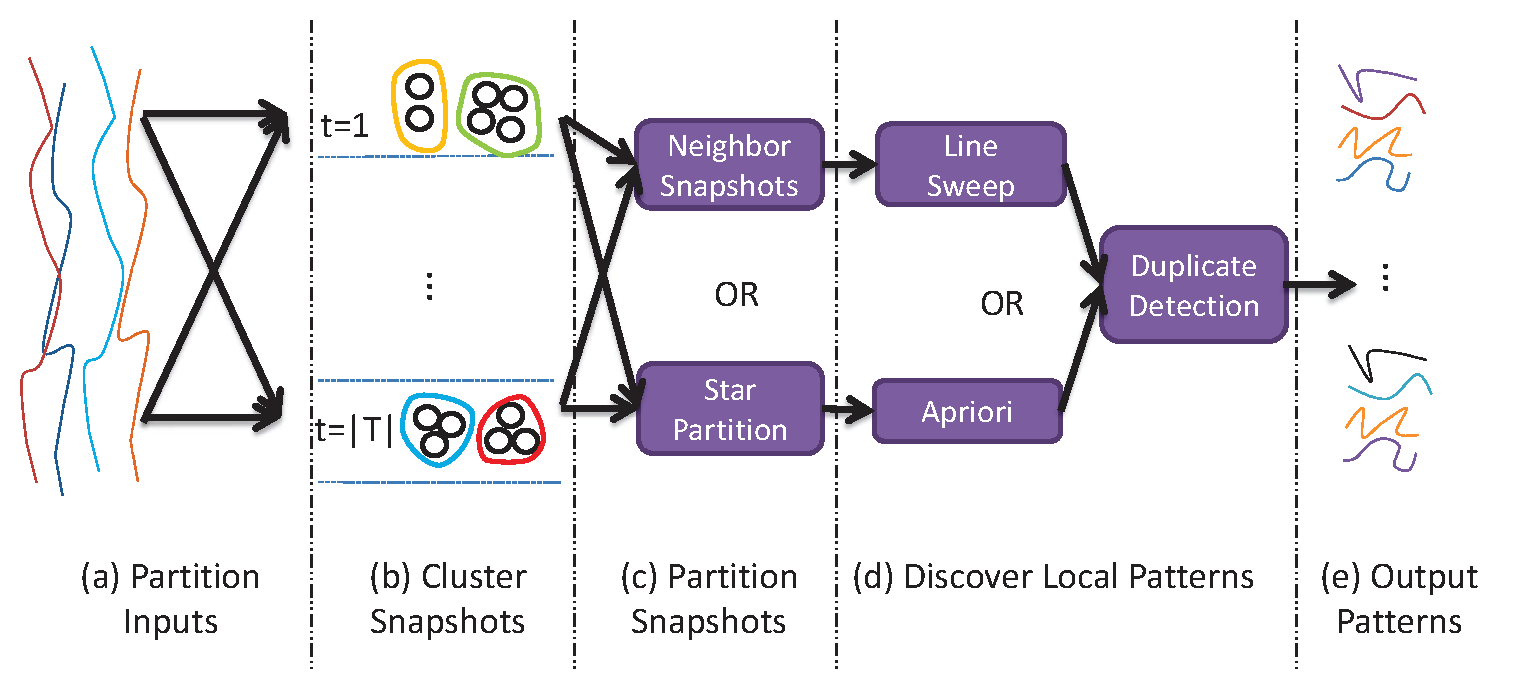
\includegraphics[width=0.5\textwidth]{system_layout.eps}
%\caption{System flow of mining GCMP. (a)(b) correspond to the first MR job which compute the clusters at each snapshot; 
%(c)(d) correspond to the second MR jobs which mines GCMP in parrallel.}
%\label{fig:overview}
%\end{figure}
%
%We note that the first MR job is easy to design since each reducer only
%needs one snapshot for clustering.
%In contrast, it is challenging to design the second job. 
%This is because valid patterns may spray across multiple snapshots 
%or contain different object sets, where inappropriate partitioning
%of snapshots may fail to discover certain valid patterns.
%Formally, a valid partition strategy 
%needs to meet the following requirements: (a) the resulted partitions need
%to preserve enough information so that real patterns can be discovered in the reduce phase. 
%(b) the resulted partitions need to ensure that
%the patterns discovered in the reduce phase are valid patterns so that
%no further verification is required. We formalize these two 
%properties as \emph{completeness} and \emph{soundness} as follows:
%
%\begin{definition}[Completeness and Soundness]
%Let a partition method $\mathbb{P}$ partitions original trajectories $Tr$ into multiple parts, $Par_1,...,Par_m$. $\mathbb{P}$ is complete if for every pattern $P$ that is valid in $Tr$, $\exists Par_i$ s.t. $P$ is valid in $Par_i$. $\mathbb{P}$ is sound if for all patterns that are valid in any $Par_i$, they are also valid in $TR$.
%\end{definition}
%The completeness ensures that no true patterns are missed out. 
%The soundness ensures that no false patterns are reported. 
%If a partition method is both sound and complete, then it can be used
%in the second MR job to facilitate GCMP mining.
%
%Apparently, replicating the entire trajectories to each 
%partition meets the \emph{soundness} and \emph{completeness} requirements. 
%However, it burdens the network shuffle and limits the parallelism. 
%Our objective is thus to design a complete and sound partition method that minimize the network shuffles.
%In the following sections, we describe a naive \emph{temporal-based} partition-and-mining method called \emph{Temporal Replication and Mining}(TRM) towards a parallel solution of GCMP mining. Then,
%we present a novel \emph{object-based} partition-and-mining method
%called \emph{Star Partition and Mining} (SPM) which resolves
%the deficiencies of TRM method.



\section{Introduction}
The prevalence of positioning devices has drastically boosted 
the scale and spectrum of trajectory collection to an unprecedented level. 
Tremendous amounts of trajectories, in the form of sequenced spatial-temporal 
records, are continually generated from animal telemetry chips, 
vehicle GPSs and wearable devices. Data analysis on large-scale 
trajectories benefits a wide range of applications and services, 
including traffic planning~\cite{zheng2011urban}, animal analysis~\cite{li2010miningperiodic}, and social recommendations~\cite{bao2013survey}, to name just a few.


A crucial task of data analysis on top of trajectories is 
to discover co-moving patterns. A \emph{co-movement} pattern~\cite{li2013managing} 
refers to a group of objects traveling together for a certain period of time 
and the group is normally determined by spatial proximity. 
A pattern is prominent if the size of the group exceeds $M$ and the length of the duration exceeds $K$, where $M$ and $K$ are parameters specified by users. Rooted from such basic definition 
and driven by different mining applications, there are a bunch of variants 
of co-movement patterns that have been developed with more advanced constraints.

Table~\ref{tbl:existing_co_patterns} summarizes several popular co-moving pattern s 
with different constraints in the attributes of clustering in spatial proximity,
consecutiveness in temporal duration and computational complexity. 
In particular,  the \emph{flock}~\cite{gudmundsson2006flock} 
and the \emph{group}~\cite{wang2006grouppattern} patterns require 
all the objects in a group to be enclosed by a disk with radius $r$; 
whereas the \emph{convoy}~\cite{jeung2008convoy}, the \emph{swarm}~\cite{li2010swarm} 
and the \emph{platoon}~\cite{li2015platoon} patterns resort to density-based 
spatial clustering. 
In the temporal dimension, the \emph{flock}~\cite{gudmundsson2006flock} 
and the \emph{convoy}~\cite{jeung2008convoy} require all the timestamps 
of each detected spatial group to be consecutive, which is referred to as \emph{global consecutiveness}; 
whereas the \emph{swarm}~\cite{li2010swarm} does not impose any restriction. 
The \emph{group}~\cite{wang2006grouppattern} and the \emph{platoon}~\cite{li2015platoon} adopt a compromised manner by allowing
arbitrary gaps between the consecutive segments, which is called \emph{local consecutiveness}. 
They introduce a parameter $L$ to control the minimum length of each local consecutive segment.


\begin{table} \scriptsize
\centering
\begin{tabular}{|c|c|c|c|}
\hline 
Patterns & {\tiny Proximity} & {\tiny Consecutiveness} & {\tiny Time Complexity}\\ 
\hline 
flock~\cite{gudmundsson2004flock} & disk-based &  global & $O(|\mathbb{O}||\mathbb{T}|(M + log(|\mathbb{O}|))$ \\ 
\hline 
convoy~\cite{jeung2008convoy} & density-based &   global & $O(|\mathbb{O}|^2+|\mathbb{O}||\mathbb{T}|)$\\ 
\hline 
swarm~\cite{li2010swarm} & density-based  & - & $O(2^{|\mathbb{O}|}|\mathbb{O}||\mathbb{T}|)$  \\ 
\hline 
group~\cite{wang2006grouppattern} & disk-based &  local & $O(|\mathbb{O}|^2|\mathbb{T}|)$ \\ 
\hline 
platoon~\cite{li2015platoon} & density-based &  local & $O(2^{|\mathbb{O}|}|\mathbb{O}||\mathbb{T}|)$\\ 
\hline 
\end{tabular} 
\caption{Constraints and complexity of co-movement patterns. The time complexity indicates the performance in the worst case, where $|\mathbb{O}|$ is the total number of objects and $|\mathbb{T}|$ is the number of descritized timestamps.}
\label{tbl:existing_co_patterns}
\end{table}




\begin{figure}[h]
\centering
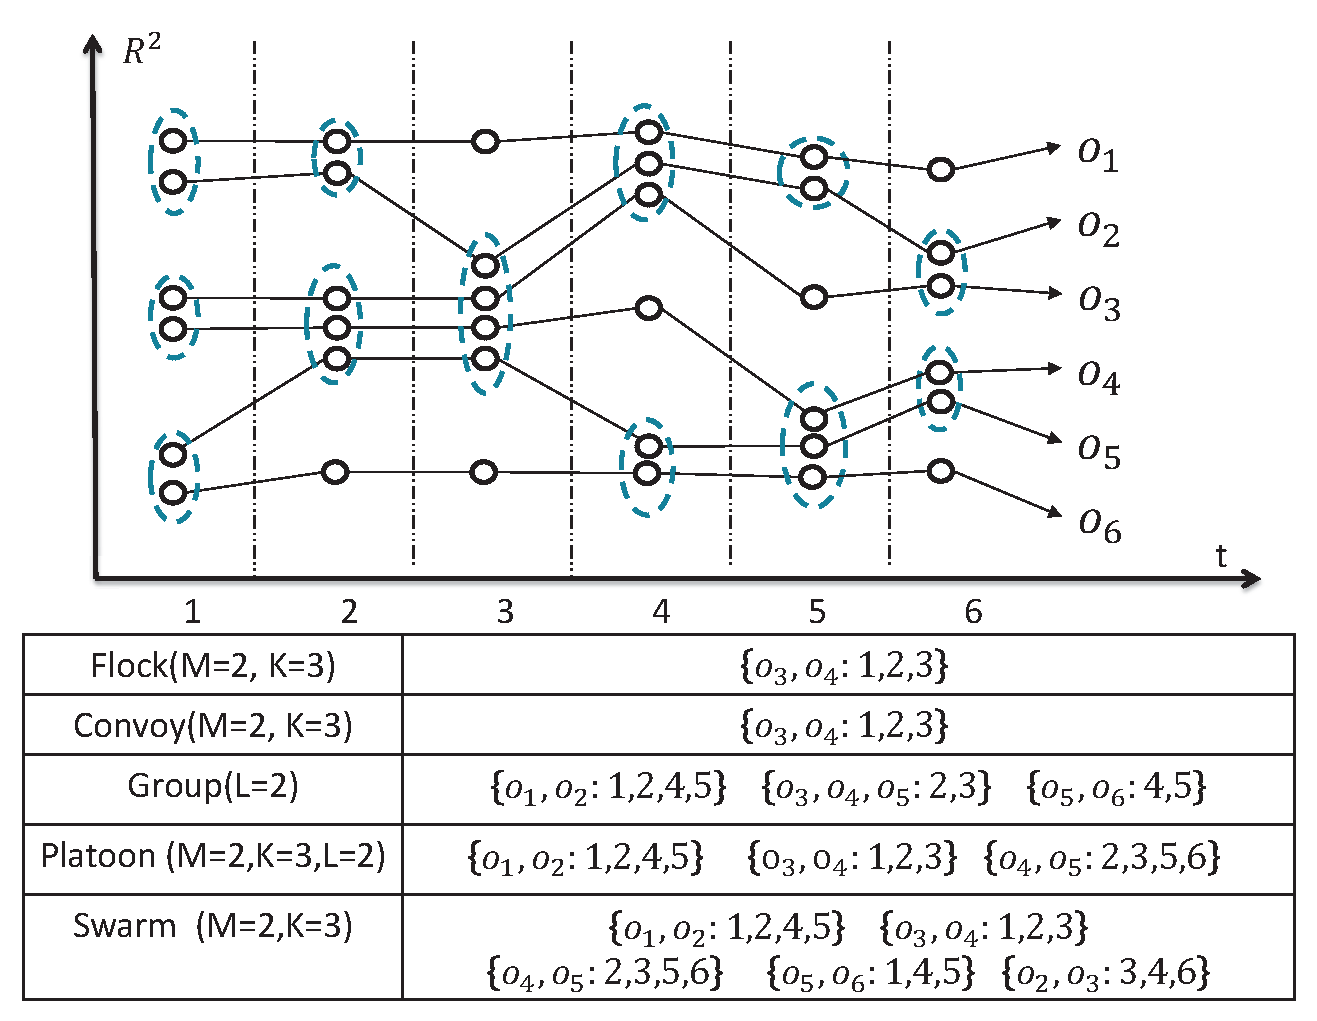
\includegraphics[width=0.45\textwidth]{related_work.eps}
\caption{Trajectories and co-movement patterns; The example consists of six trajectories across six snapshots. Objects in spatial clusters are enclosed by dotted circles. $M$ is the minimum cluster cardinality; $K$ denotes the minimum number of snapshots for the occurrence of a spatial cluster; and $L$ denotes the minimum length for local consecutiveness.}
\label{fig:related_work}
\end{figure}

Figure~\ref{fig:related_work} is an example to demonstrate the concepts of various co-movement patterns. The trajectory database consists of six moving objects and the temporal dimension is discretized into six snapshots. In each snapshot, we treat the clustering methods as a black-box and assume that they generate the same clusters. Objects in proximity are grouped in the dotted circles. As aforementioned, there are three parameters to determine the co-movement patterns and the default settings in this example are $M=2$, $K=3$ and $L=2$. Both the \emph{flock} and the \emph{convoy} require the spatial clusters to last for at least $K$ consecutive  timestamps. Hence,$\{o_3,o_4\}$ and $\{o_5,o_6\}$  remains the only two candidates matching the patterns. The \textit{swarm} relaxes the pattern matching by discarding the temporal consecutiveness constraint. Thus, it generates many more candidates than the \textit{flock} and the \textit{convoy}. The \textit{group} and the \textit{platoon} add another constraint on local consecutiveness to retain meaningful patterns. For instance, $\{o_1,o_2:1,2,4,5\}$ is a pattern matching local consecutiveness because timestamps $\{1,2\}$ and $\{4,5\}$ are two segments with length no smaller than $L=2$. The difference between the \textit{group} and the \textit{platoon} is that the \textit{platoon} has an additional parameter $K$ to specify the minimum number of snapshots for the spatial clusters. This explains why $\{o_3,o_4,o_5:2,3\}$ is a  \textit{group} pattern but not a \textit{platoon} pattern.

As can be seen, there are various co-movement patterns requested by different applications and it is cumbersome to design a tailored solution for each type. In addition, despite the generality of the \emph{platoon} (i.e., it can be reduced to other types of patterns via proper parameter settings), it suffers from the so-called \emph{loose-connection} anomaly. We use two objects $o_1$ and $o_2$ in Figure~\ref{fig:platoon_weakpoint} as an example to illustrate the scenario. These two objects form a \emph{platoon} pattern in timestamps $\{1,2,3,102,103,104\}$. However, the two consecutive segments are $98$ timestamps apart, resulting in a false positive co-movement pattern. In reality, such an anomaly may be caused  by the periodic movements of unrelated objects, such as vehicles stopping at the same petrol station or animals pausing at the same water source. 
Unfortunately, none of the existing patterns have directly addressed this anomaly.


%As can be seen, there are various co-movement patterns requested by different 
%applications and it is cumbersome to design a tailored solution for each type. 
%As pointed in \cite{li2015platoon, li2010swarm}, stringent temporal constraints (e.g., global consecutiveness on \emph{flock} and \emph{convoy}) may miss out many interesting patterns. However, we 
%further observe that pattern definitions with overly-relaxed temporal constraints (e.g., \emph{swarm}, \emph{group} and \emph{platoon}) lose the fine control of a pattern which lead to noisy results and unnecessary computations. We name this scenario as \emph{loose-connection} anomaly. To illustrate, as shown in Figure~\ref{fig:platoon_weakpoint}, the two objects $o_1, o_2$ form a \emph{platoon} pattern 
%$\{o_1,o_2:1,2,3,102,103,104\}$. However, the consecutive segments are $98$ timestamps apart, 
%making the co-moving behavior very loose.
%In reality, such an anomaly is likely induced by the periodic movements of unrelated objects 
%such as, vehicles stopping at the same petrol station, animals pausing at the same water source etc.  Interestingly, none of the temporal-relaxed patterns (e.g., \emph{swarm}, \emph{group} and \emph{platoon}) are able to directly avoid such an anomaly.

%In addition, existing pattern definitions are not expressive enough and may miss 
%interesting patterns or return noisy results. We summarize 
%the two scenarios as \emph{missing-pattern} anomaly
%and \emph{loose-connection} anomaly.
%A \emph{missing-pattern} anomaly arises due to the stringent constraints on the pattern duration.
%As shown in Figure~\ref{fig:platoon_weakpoint} (a), if we set $K=4$, 
%neither \emph{flock}s nor \emph{convoy}s can be discovered. This is because
%$o_1$ is away from $o_2$ at timestamp $4$, which is likely caused by
%the traffic control or the clustering inaccuracy at time $4$. On the other hand,
%the \emph{loose-connection} anomaly occurs due to an over-relaxed constraint on 
%the duration. As shown in Figure~\ref{fig:platoon_weakpoint} (b),
%the two objects $o_1, o_2$ form a \emph{platoon} pattern 
%$\{o_1,o_2:1,2,3,102,103,104\}$. However, the consecutive segments are $98$ timestamps apart, 
%making the co-moving behavior very weak.
%In reality, such an anomaly is likely to be induced by the periodic movements of unrelated objects 
%such as, vehicles stopping at the same petrol station, animals pausing at the same water source etc. 
%It is easy to see that none of the existing co-movement patterns are able to avoid these two anomalies.

\begin{figure}[h]
\center
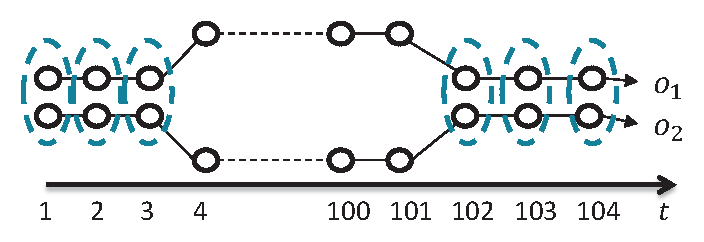
\includegraphics[width=0.35\textwidth]{platoon_weakpoint.eps}
\caption{\emph{Loose-connection} anomaly. Even though $\{o_1, o_2: 1,2,3,102,103,104\}$ is considered as a valid \emph{platoon} pattern, it is highly probable that these two objects are not related as the two consecutive segments  are 98 timestamps apart. 
% in \emph{platoon}, \emph{swarm} and \emph{group} results.
}
\label{fig:platoon_weakpoint}
\end{figure}

%In current literature,
%users are unable to explicitly exclude the loosely-connected patterns even when those patterns are unwanted.
%
%
% we summarize two anomalies 
%The \emph{missing-pattern}~\cite{li2010swarm} anomaly arises due to the stringent constraints on the duration of a pattern. As shown in 
%Figure~\ref{fig:platoon_weakpoint} (a).  As we notice, object $o_1$ is temporally far from $o_2$ at timestamp $4$, which is likely to be
%the result of errors in interpretation of missing points, or $o_1$ faces traffic control at time $4$. Such an anomaly can
%be resolved by \emph{swarm} and \emph{platoon} due to a relaxed constraint on the duration. However, 
%\emph{swarm} and \emph{platoon}'s relaxations encompass a type of non-interesting patterns which is referred
%as \emph{loose-connection}~\cite{li2015platoon} anomaly. 
%
%
%%This is because that \emph{platoon} allows the timestamps in a pattern duration to be in arbitrary distance, making the object group loosely
%connected. For instance, patterns with duration $\{1,2,100,101\}$ could be a valid \emph{platoon}; however, the two timestamps $2,100$ are too far from each other.

%For instance, PUT THE FIGURE AND EXPLANATION HERE.

%\begin{figure}[h]
%\center
%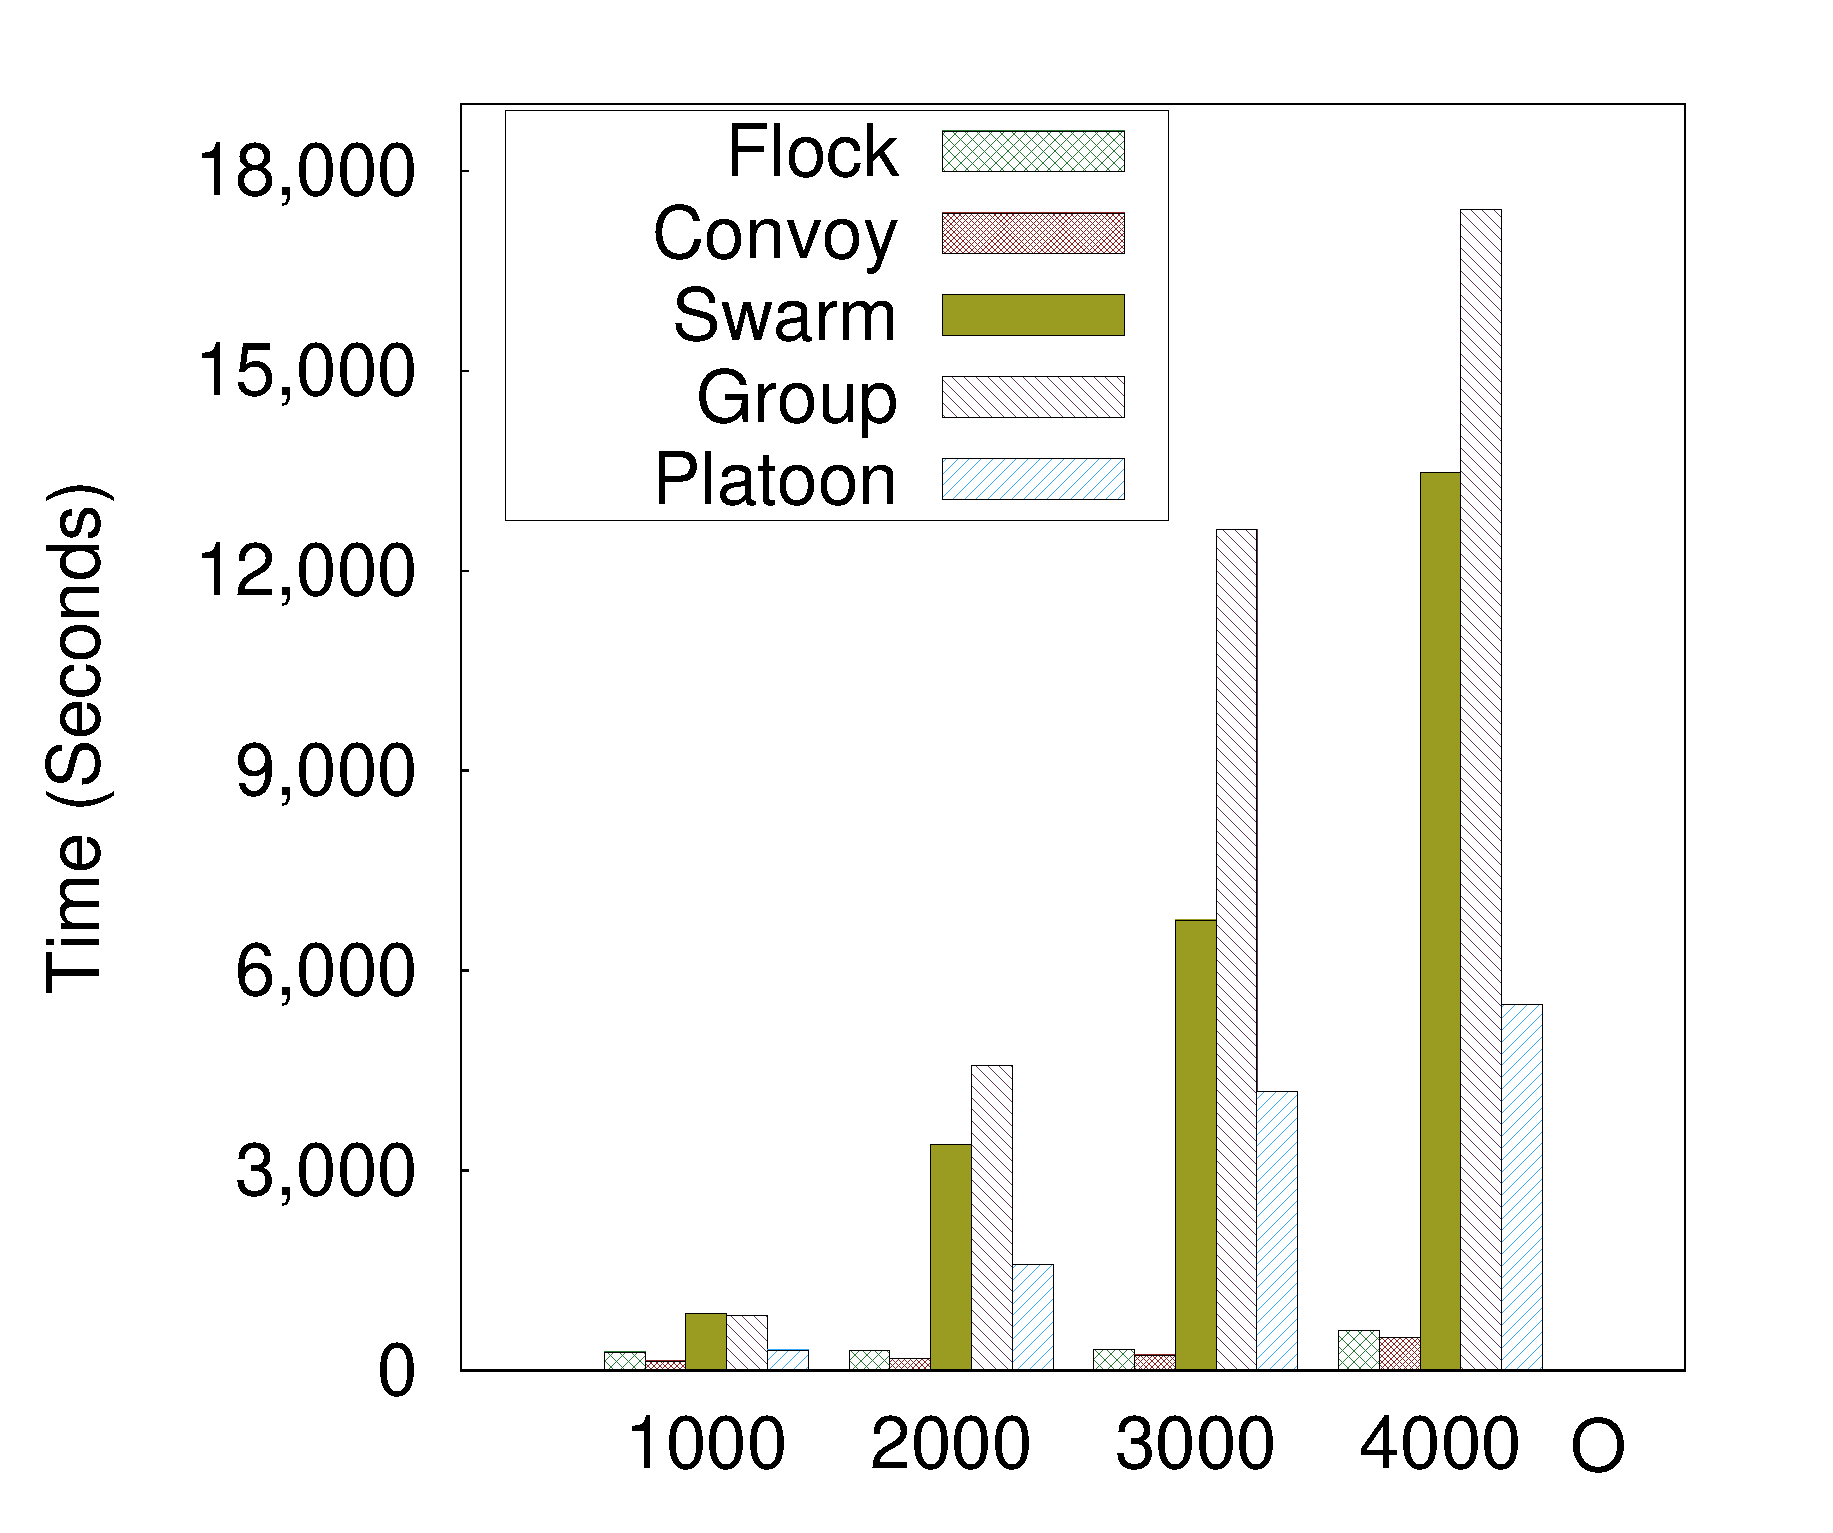
\includegraphics[width=0.35\textwidth]{rw_perf_O.eps}
%\caption{Two anomalies in existing patterns. (a) \emph{Missing-pattern} anomaly
%in \emph{flock} and \emph{convoy}. When $K=4$, none of the two patterns can be discovered. (b) \emph{Loose-connection} anomaly in \emph{platoon} and \emph{swarm}. The consecutive segment of $o_1$ and $o_2$ are 98 timestamps apart, however, the pattern $\{o_1, o_2: 1,2,3,102,103,104\}$ is included in platoon and swarm results.}
%\label{fig:platoon_weakpoint}
%\end{figure}


The other issue with existing methods is that they are built on top of centralized indexes which may not be scalable. Table~\ref{tbl:existing_co_patterns} shows their theoretical complexities in the worst cases and the largest real dataset ever evaluated in previous studies is up to million-scale points collected from hundreds of moving objects. In practice, the dataset is of much higher scale and the scalability of existing methods is left unknown. Thus, we conduct an experimental evaluation with $4000$ objects moving for $2500$ timestamps to examine the scalability. Results in Figure~\ref{fig:related_work_scalability} show that their performances degrade dramatically as the dataset scales up. For instance, the detection time of \emph{group} drops twenty times as the number of objects grows from \emph{1k} to \emph{4k}. Similarly,
the performance of \emph{swarm} drops over fifteen times as the number of snapshots grows from \emph{1k} to \emph{2.5k}.
These observations imply that existing methods are not scalable to support large-scale trajectory databases. 

%It is easy to spot that none of the existing solutions are scalable to handle large-scale trajectories which include near billions of data points.
%In fact, as shown in Table~, the mining of co-movement patterns require high complexity. For instance, the
%complexities of \emph{swarm} and \emph{platoon} are already exponential. 
%Therefore, none of them can handle millions of trajectories efficiently. 
%CAN YOU ANALYSE THEIR COMPLEXITY TO ADDRESS THE PROBLEM OF SCALABILITY.
\begin{figure}[h]
    \centering
    \begin{subfigure}[b]{0.23\textwidth}
            \centering
            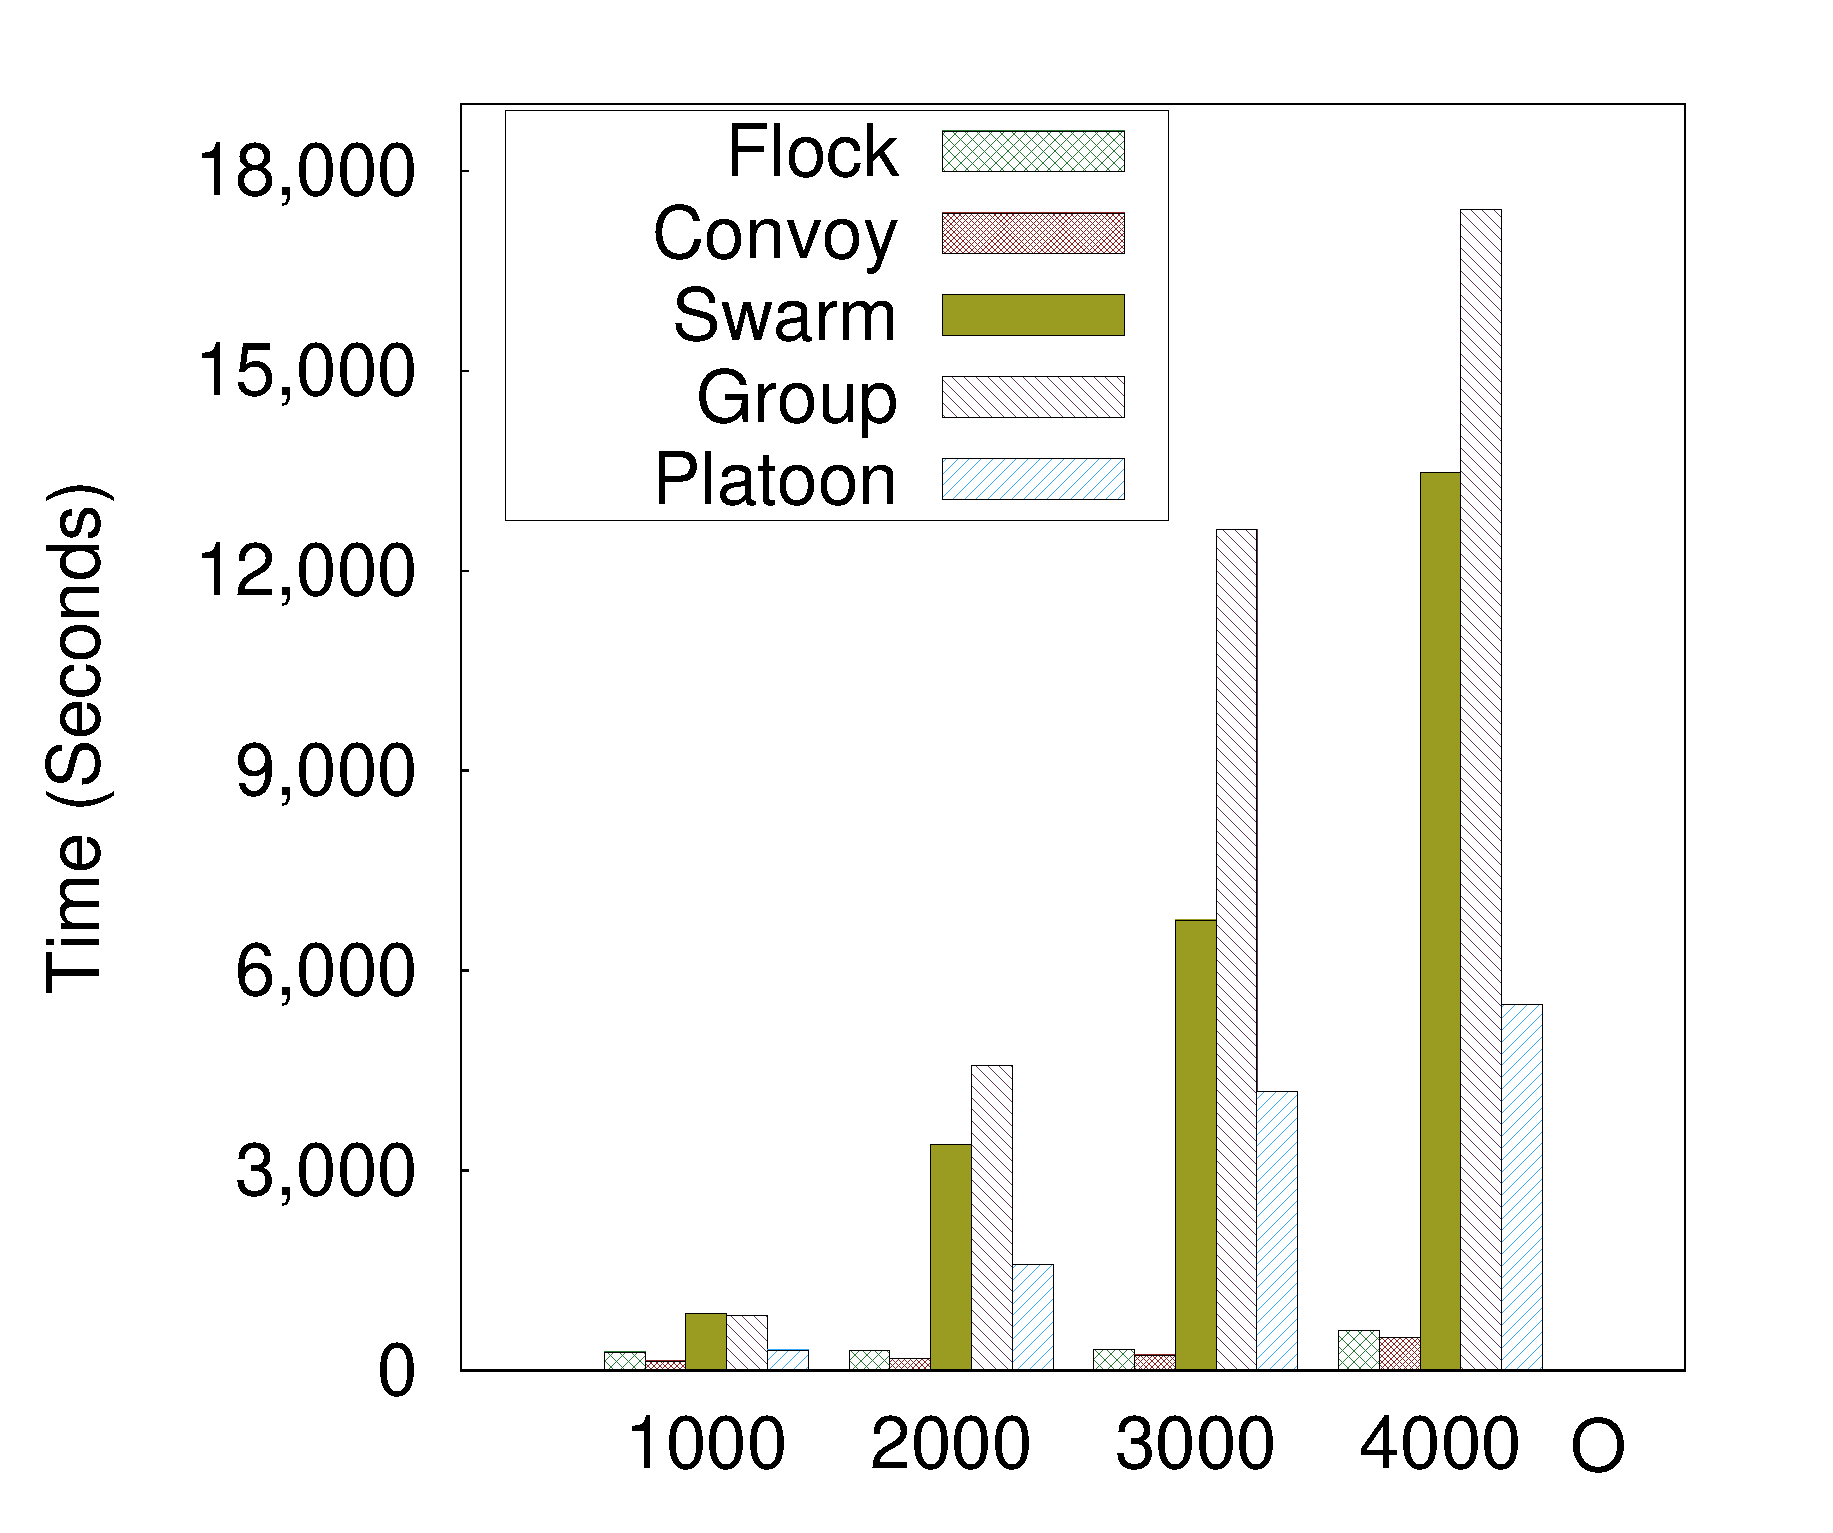
\includegraphics[width=\textwidth]{rw_perf_O.eps}
		\subcaption{$1k$ timestamps}
    \label{fig:fig1}
    \end{subfigure}
    \begin{subfigure}[b]{0.23\textwidth}
            \centering
            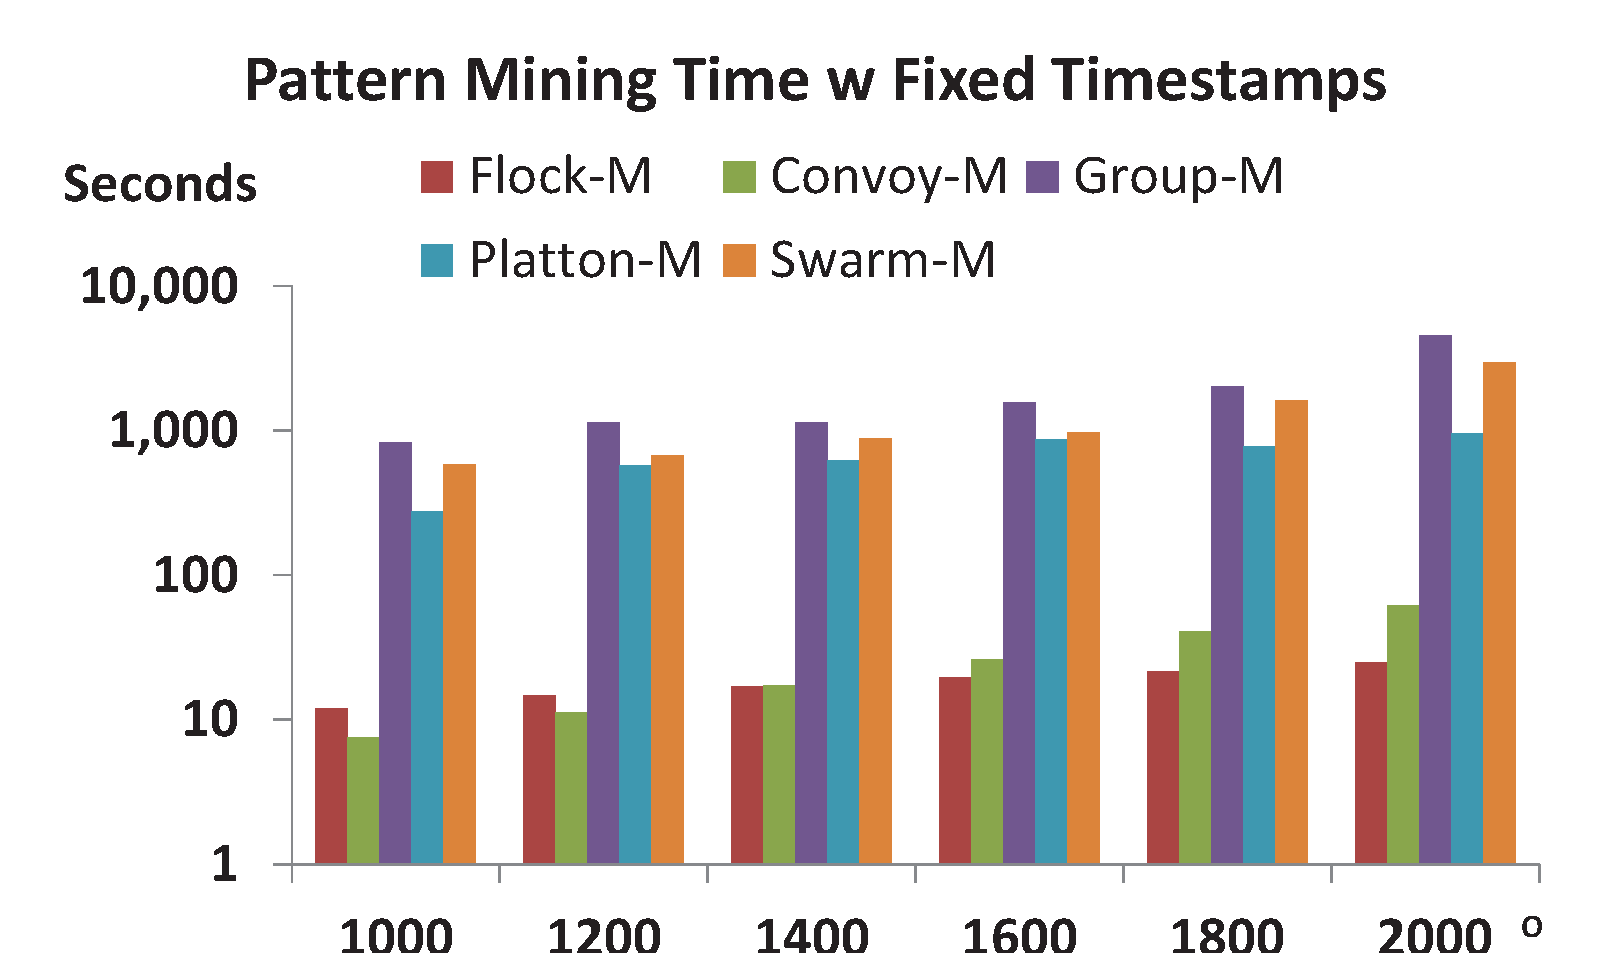
\includegraphics[width=\textwidth]{rw_perf_T.eps}
         \subcaption{$1k$ objects}
    \label{fig:fig2}
    \end{subfigure}
    \caption{Performance measures on existing co-movement patterns. A sampled Geolife data set
    is used with up two 2.4 million data points. Default parameters are $M=10$ $K=20$ $L=10$.}
    \label{fig:related_work_scalability}
\end{figure}




Therefore, our primary contributions in this paper are to close these two gaps. 
First, we propose the \emph{general co-movement pattern} (GCMP) which models
various co-moment patterns in a unified way and can avoid 
the \emph{loose-connection} anomaly. In GCMP, we introduce a new gap parameter $G$ to pose a constraint on the temporal gap between two consecutive segments. By setting a feasible $G$, the loose-connection anomaly can be avoided. In addition, our GCMP is both general and expressive. It can be reduced to any of the previous patterns by customizing the parameters.

%Therefore, users are 
%still able to exclude non-consecutive patterns 
%or include loosely-connected patterns when they feel necessary.


%We introduce the gap parameter $G$,
%When such loosely-connected patterns are unwanted, users currently are unable to directly control the outputs.
%To cope with both of the two anomalies, we propose 
%by introducing the gap parameter $G$, 

%By so doing, we gain a fine-grained control s, which As we show in later sections, the general co-movement pattern is able to express existing patterns by setting appropriate parameters. 
%IS IT POSSIBLE TO USE FIGURE 1 TO ADDRESS THE PROBLEM OF PLATOON, INSTEAD OF PROPOSING A NEW EXAMPLE SCENARIO?
%

Second, we investigate deploying our GCMP detector on MapReduce platforms (such as Hadoop and Spark) to tackle the scalability issue. Our technical contributions are three-fold. First, we replicate the snapshots in multiple data chunks to support efficient parallel processing. Second, we devise a novel \emph{Star Partition and Mining} (SPM) algorithm as a fine-granularity partitioning strategy to achieve workload balance. For each star, an Apriori method is adopted to mine the co-movement patterns. Third, we leverage the \emph{temporal monotonicity} property of GCMP to design several optimization techniques including \emph{edge-simplification} to prune initial candidates, \emph{temporal apriori pruning} and \emph{forward closure checking} to reduce the number of enumerated candidates in the Apriori algorithm.
%
%we propose two types of optimization techniques to further improve the performance, including \emph{edge-simplification} to boost the shuffle process and \emph{temporal monotonicity pruning} and 
%\emph{forward closure checking} to significantly reduce the number of enumerated candidates in the Aproiro algorithm.


We conduct a set of extensive experiments on three large-scaled real datasets with hundreds of millions 
temporal points. 
The results show that our parallel scheme efficiently supports GCMP mining in large datasets.
In particular, with near 200 million trajectory points, 
our scheme runs within 10 minutes using 135 cores. Whereas centralized solution takes near 7 hours for 
1 million trajectory points.
Moreover, our optimized SPM methods achieves upto XXX times efficiency
as compared to the baseline algorithm with near linear scalability.

The rest of our paper is organized as follows: Section~\ref{sec:related_works} summarizes the relevant literature on 
trajectory pattern mining. Section~\ref{sec:definition} states the problem definition of our general co-movement pattern mining. Section~\ref{sec:trm} provides a baseline solution. An advanced solution named
\emph{star partition and mining} is presented in Section~\ref{sec:spm}. Section~\ref{sec:opt} discusses various optimization techniques. Section~\ref{sec:exp} conducts extensive experiments to verify the efficiency of our system. Finally Section~\ref{sec:concl} concludes the paper.

\section{Related Works}
\label{sec:related_works}
The \emph{co-movement patterns} in literature consist 
of five members, namely \emph{group}~\cite{wang2006grouppattern}, \emph{flock}~\cite{gudmundsson2004flock},
\emph{convoy}~\cite{jeung2008convoy}, \emph{swarm}~\cite{li2010swarm} and \emph{platoon}~\cite{li2015platoon}.
We have demonstrated the semantics of these patterns in Table~\ref{tbl:existing_co_patterns} and Figure~\ref{fig:related_work}.
In this section, we focus on comparing the techniques used in these works. 
%Another related area to our work is \emph{Trajectory Clustering}, we summarize several of the representative techniques in the later part of the section. 
For more trajectory patterns other than \emph{co-movement patterns}, 
interested readers may move to~\cite{zheng2015survey} for a comprehensive survey.

%The \emph{Co-movement Pattern} belongs to the area of 
%\emph{Spatio-Temporal Pattern} in trajectory mining where many research works are spawned.
%In this section, we only focus on two closest area of literature namely \emph{Co-Movement Pattern Mining}
%and \emph{Trajectory Clustering}. As far as we know, there is little research
%works on providing parallel solutions to \emph{Co-Movement Pattern} mining. 

\subsection{Flock and Convoy}
The difference between \emph{flock} and \emph{convoy} lies 
in the object clustering methods. In \emph{flock}
objects are clustered based on their distance. Specifically, the
objects in the same cluster needs to have a pair-wised distance less than \emph{min\_dist}. 
This essentially requires the objects to be within a disk-region of delimiter less than \emph{min\_dist}.
In contrast, \emph{convoy} cluster the objects using density-based clustering~\cite{birant2007st}.
Technically, \emph{flock} utilizes a $m^{th}$-order Voronoi diagram~\cite{laube2005finding} to detect whether
a subset of object with size greater than $m$ stays in a disk-region. \emph{Convoy} employs
a trajectory simplification~\cite{douglas1973trajectorysimplification} technique to boost pairwise distance computations in
the density-based clustering.
After clustering, both \emph{flock} and \emph{convoy} use a line-sweep 
method to scan each snapshots. During the scan, the object
group appears in consecutive timestamps is detected. Meanwhile, the object groups that do not
match the consecutive constraint are pruned. 
However, such a method faces high complexity issues when supporting other patterns.
For instance, in \emph{swarm}, the candidate set during the line-sweep grows
exponentially, and many candidates can only be pruned after the entire snapshots are scanned.

\subsection{Group, Swarm and Platoon}
Different from \emph{flock} and \emph{convoy}, all the \emph{group},\emph{swarm} and \emph{platoon}
patterns have more constraints on the pattern duration. Therefore, their techniques of mining are of
the same skeleton. The main idea of mining is to grow object set from an empty set
in a depth-first manner. During the growth, various pruning techniques are provided to prune 
unnecessary branches. \emph{Group} pattern uses the Apriori property among patterns to facilitate the pruning.
\emph{Swarm} adapts two more pruning rules called backward pruning and forward pruning. \emph{Platoon}
further adapts a prefix table structure to guide the depth-first search. As shown by Li et.al.~\cite{li2015platoon},
\emph{platoon} outperforms other two methods in efficiency. 
However, the three patterns are not able to directly discover the general co-movement pattern.
Furthermore, their pruning rules heavily rely on the depth-first search nature, which lost its efficiency
in the parallel scenario.

THESE WORKS ARE MOST RELATED TO OUR PROBLEMS, SO I REMOVED OTHER RELATED WORKS FOR NOW. 

%\subsection{Platoon Pattern}
%Li et. al.~\cite{li2015platoon} design a prefix table based pruning rule for fast compute Platoon Pattern.

%\subsection{Trajectory Clustering}
%Another related field is trajectory clustering~\cite{he2011mrdbscan,lee2007partitionandgroup,
%li2004clusteringmovingobjects}. Lee et al. proposed a partition and group algorithm in~\cite{lee2007partitionandgroup}
%to discover trajectories segments of similar geometric layout.
%Their clustering method does not consider the temporal constraint so the patterns discovered
%are not \emph{Co-Movement} patterns.
%
%Li et al. proposed a \emph{micro-clustering} technique~\cite{li2004clusteringmovingobjects} to cluster moving objects based on their moving directions. However, its distance measured is defined upon the entire trajectory and cannot be applied in our problem to mine local patterns.
%
%In ~\cite{he2011mrdbscan}, He et al. deployed an implementation of DBSCAN on MapReduce. They decouple the dependency of original DBSCAN algorithm into a four-stage parallel process.  However their method only focuses on DBSCAN for one snapshot, where exploiting the relationship between multiple DBSCANs remains unexplored. I DON'T UNDERSTAND WHAT YOU MEAN. ONE DATASET? MULTIPLE DBSCANS?
%
%Trajectory pattern mining can be roughly classified into four categories, 
%namely \emph{Co-Movement Pattern Mining}, \emph{Frequent Sequence Mining},
%\emph{Trajectory Clustering} and \emph{Periodic Pattern Mining}. The most
%relevant literature to our work is \emph{Co-Movement Pattern Mining}. In this
%section, we focus on summarizing existing works on \emph{Co-Movement Pattern Mining}. 
%Interested readers may refer to~\cite{} for a comprehensive survey on 
%other types of trajectory mining techniques.


%The relevant literature can be classified into three groups, namely \emph{Co-Movement Patterns},
%\emph{Spatio Patterns} and \emph{Parallel Trajectory Processing Platforms}
%
%In this section, we present a comprehensive literature review on the related works. 

%\subsection{Co-movement Pattern}
%
%FOR THE CO-MOVEMENT PATTERN, YOU NEED TO EMPHASIZE TWO THINGS: 1) THE DIFFERENCE BETWEEN PATTERNS. NEED TO CLARIFY THE PARAMETERS IN EACH MODEL. 2) CLEARLY STATE THE MINING TECHNIQUES. 
%\subsection{Co-movement Pattern}
%The work most related to ours is those on \emph{co-movement} patterns. We summarize the typical patterns as follows:
%\subsubsection{group}
%Wang et al. defined \emph{group pattern}~\cite{wang2006grouppattern}, which aims to find the set of objects travelling together at certain time intervals. In \emph{group pattern}, groups at each snapshot is identified by a disc-based clustering method, where each cluster forms a circle within a radius. It is argued in later works~\cite{jeung2008convoy,li2010swarm} that such disc-based clustering is not effective as \emph{density}-based clustering where the later one may find clusters of arbitrary shapes.
%
%\subsubsection{flock}
%Gudmunsson et al. proposed \emph{flock} pattern in 
%\cite{gudmundsson2004flock,gudmundsson2006flock} and Vieria et al. followed up with an online version in~\cite{
%vieira2009onlineflock}. A \emph{flock} pattern tries to find the set of objects that stay in a circular ranged cluster for a minimum duration. Such a pattern is useful in detecting the moving companions. However, similar as \emph{group pattern}, it uses disc-based clustering, which suffers the same deficiency in discovering arbitrary shaped clusters. \emph{Flock} pattern has many derivatives. In \cite{benkert2006meet}, Benkert et al. studied \emph{meet} pattern, which require the clusters in the pattern to be geographically stationary. Giannotti et al. studied \emph{leadership} pattern~\cite{andersson2007leadership} which requires a leader object exists for each flock cluster.
%
%%In \cite{benkert2006meet}, Benkert et al. studied \emph{meet} pattern. A \emph{meet} pattern aims to find a set of objects stay
%%stationary with in a circular range for some durations. This pattern does not consider the temporal movement of objects. Giannotti et al. studied \emph{leadership} pattern~\cite{andersson2007leadership} which requires a set of objects stay relatively within a circular range at each snapshots for some durations and there is at least one object is heading (leader). It is shown in~\cite{giannotti2007survey} that both \emph{Meet} and \emph{leadership} patterns are special cases of the \emph{flock} pattern~\cite{gudmundsson2004flock}.
%
%
%
%\subsubsection{convoy}
%Jeung et al. proposed \emph{convoy} pattern that extends \emph{flock} pattern by replacing the disc-based clustering with \emph{density}-based clustering. Such an relaxation brings a high complexity of repeatedly running DBSCAN~\cite{birant2007st} at every snapshot. To reduced the complexity, Jeung et al. designed a filter-refine approach which first uses simplification technique~\cite{douglas1973linesimplification} to filter far away objects, and then uses coherent moving method~\cite{kalnis2005movingclusters} to find the exact convoy patterns. Along with \emph{convoy} pattern, Aung et al. proposed \emph{dynamic convoy} and \emph{evolving convoy} patterns. In \emph{dynamic convoy}, the cluster members are allowed to be absent briefly during the convoy lifetime, while \emph{evolving convoy} allows the convoy to grow or shrink in cardinality during the life time. Tang et al. also addresses the online extension in~\cite{tang2012onlineconvoy}.
%\subsubsection{swarm}
%The major argument on \emph{convoy} pattern is that \emph{convoy} requires the consecutiveness in the lifetime, which may lose many interesting patterns. To remedy, Li et al. proposed the \emph{swarm} pattern~\cite{li2010swarm} which completely relaxes the consecutiveness in \emph{convoy}. In \emph{swarm}, objects can collectively leave the cluster for a long time and then join back in later time. The only requirement in \emph{swarm} is that each member in the cluster needs to accumulate to a certain duration. In~\cite{li2010swarm}, the authors proposed a depth-first search based pruning algorithm to efficiently discover \emph{swarm} patterns.
%\subsubsection{platoon}
%Recently Li et al. argued that \emph{swarm} is to loose in the temporal consecutiveness and proposed \emph{platoon} pattern in~\cite{li2015platoon}. In \emph{platoon} pattern, the clusters should lasts for at least a certain during before dismiss. Meanwhile, \emph{platoon} allow the clusters to form again at future times. Li et al. demonstrated the such extension is more general and can support swarm and convoy patterns by setting appropriate parameters. Li et al. also provide a similar depth-first search approach as in~\cite{li2010swarm}. In addition, they adapted a prefix pruning method to further improve efficiency. It is notable that in both \cite{li2010swarm} and \cite{li2015platoon}, authors consider the input to be the clusters at each snapshot, which ignores the clustering time.
%
%\subsection{Other Related Trajectory Patterns}
%Besides co-movement patterns, there are a number of other types of trajectory patterns proposed in previous works.
%%General Trajectory pattern mining a hot field in trajectory analysis. Previous works
%%define various patterns~\cite{
%%kalnis2005movingclusters,
%%li2010periodicpattern,zheng2013gathering,jinno2012paralleltpattern,li2013onlinegroup} over trajectory data, which have proven their usefulness under different applications~\cite{giannotti2007survey}. 
%
%Kalnis et al. proposed \emph{moving clusters} pattern~\cite{kalnis2005movingclusters}. In such a pattern, objects form clusters at each snapshot. For consecutive snapshots, the clusters in the pattern should have a Jaccard index greater than a threshold. Under such a scheme, the difference between cluster members in snapshots accumulates, therefore the clusters at later snapshot may be very different from those in previous snapshots. The online extension is studied by Li et al.~\cite{li2013onlinegroup}. IT'S DIFFERENCE WITH CO-MOVEMENT PATTERN IS NOT CLEAR. WHAT IS JACCARD INDEX?
%
% In~\cite{li2010periodicpattern}, Li et al. studied the \emph{periodic} pattern, which mines objects with periodic behaviors. 
%It is commented in~\cite{giannotti2007survey} that \emph{periodic} pattern is unsuitable for discovering movements, since it is unreasonable to expect an object to repeat its behavior exactly during each time period considered. AGAIN, WHAT'S YOUR POINT? YOU MEAN SUCH A WORK IS MEANINGLESS? THEN, WHY BOTHER TO MENTION IT HERE?
%
%Zhang et al. proposed the \emph{gathering} pattern in \cite{zheng2013gathering}. It is similar to \emph{flock} pattern~\cite{gudmundsson2004flock} but with the relaxation on the members of clusters. Instead of fixing the members in clusters as in~\cite{gudmundsson2004flock}, \emph{gathering} pattern allows members in clusters leave and join during the pattern duration. Since it relaxes the member constraints, it is unable to model co-movement patterns. HOW TO DEFINE CO-MOVEMENT PATTERN? IS THERE A PREVIOUS ``FORMAL'' DEFINITION? OR IS DEFINED BY YOU? THIS ONE LOOKS LIKE OBJECTS CO-MOVE. WHY IT IS NOT A CO-MOVEMENT PATTERN?
%
%
%%\subsection{Pattern Mining Frameworks}
%Jinno et al. recently studied the problem of processing \emph{T}- pattern~\cite{giannotti2007survey} in parallel platform \cite{jinno2012paralleltpattern}. A \emph{T}-pattern discovers a set of objects visiting the same the place in a close time interval. Such a pattern differs from moving object pattern in that \emph{T}-pattern does not consider the movement of objects. Jinno et al. in~\cite{jinno2012paralleltpattern} designed a MapReduce based algorithm for efficiently support \emph{T}-pattern discovery. However, as the nature of differences between the patterns, their work cannot directly applied on the co-moving object pattern discovery. Li et al. recently proposed a framework of processing online \emph{evolving group} pattern~\cite{li2013onlinegroup}. The \emph{evolving group} is similar to \emph{moving cluster} pattern with focus on the member updates in clusters, which is different with \emph{co-movement} pattern. Moreover the framework is developed for centralized system, thus is different with our work.
%
%\subsection{Trajectory Clustering}
%Another related field is trajectory clustering~\cite{he2011mrdbscan,lee2007partitionandgroup,
%li2004clusteringmovingobjects}. Lee et al. proposed a partition and group algorithm in~\cite{lee2007partitionandgroup} TO SOLVE WHAT PROBLEM?. Their clustering method does not consider the temporal constraint and groups trajectories from different time points together. WHY EMPHAISIS THIS? OUR CLUSTERING IS ALSO CONDUCTED IN EACH SNAPSHOT. 
%
%Li et al. proposed a \emph{micro-clustering} technique~\cite{li2004clusteringmovingobjects} to cluster moving objects based on their moving directions. However, its distance measured is defined upon the entire trajectory and cannot be applied in our problem to mine local patterns.
%
%In ~\cite{he2011mrdbscan}, He et al. deployed an implementation of DBSCAN on MapReduce. They decouple the dependency of original DBSCAN algorithm into a four-stage parallel process.  However their method only focuses on DBSCAN for one datasets, where exploiting the relationship between multiple DBSCANs remains unexplored. I DON'T UNDERSTAND WHAT YOU MEAN. ONE DATASET? MULTIPLE DBSCANS?
\section{Definitions}
\label{sec:definition}
Let $\mathbb{O} = \{o_1 ,o_2,...,o_n\}$ be the set of objects and $\mathbb{T} =(1,2,...,N)$ be the discretized temporal dimension. A time sequence $T$ is defined as an ordered subset of $\mathbb{T}$. Given two time sequences $T_1$ and $T_2$, we define a bunch of commonly-used operators in this paper in Table~\ref{tbl:operators}.

\begin{table}[h] \scriptsize
\centering
\begin{tabular}{|c|l|}
\hline 
\textbf{Operator} & \textbf{Definition} \\ 
\hline
$T[i]$ & the $i$-th element in the sequence $T$ \\ 
\hline
$|T|$ & the number of elements in $T$\\
\hline
$\max(T)$ & the maximum element in $T$\\
\hline
$\min(T)$ & the minimum element in $T$\\
\hline
$\range(T)$ & the range of $T$, i.e., $\max(T) - \min(T) +1$\\ 
\hline 
$T[i:j]$ & subsequence of $T$ from $T[i]$ to $T[j]$ (inclusive) \\ 
\hline
$T_1\subseteq T_2$ &  $\forall T_1[x]\in T_1$, we have $T_1[x]\in T_2$. \\\hline
$T_3=T_1\cup T_2$ & $\forall T_3[x]\in T_3$, we have $T_3[x]\in T_1$ or $T_3[x] \in T_2$\\ 
\hline
$T_3=T_1\cap T_2$ & $\forall T_3[x]\in T_3$, we have $T_3[x]\in T_1$ and $T_3[x] \in T_2$\\ 
\hline
\end{tabular}
\caption{Operators on time sequence.} \label{tbl:operators}
\end{table} 
 

We say a sequence $T$ is consecutive 
if $\forall i \in (1,...,|T|-1), T[i+1] = T[i] + 1$.  We refer each consecutive subsequence of $T$ as a \emph{segment}.
It is obvious that any time sequence $T$ can be decomposed into
segments and we say $T$ is \textit{L-consecutive}~\cite{li2015platoon} 
if the length of every segment is no smaller than $L$. As illustrated in Figure~\ref{fig:platoon_weakpoint}, patterns adopting the notion of $L$-consecutiveness (e.g., \emph{platoon} and \emph{group}) still suffer from the \emph{loose connection} problem. 
To avoid such an anomaly without losing pattern generality, we introduce a parameter $G$ to control the gaps between
timestamps in a pattern. Formally, a $G$-connected time sequence is defined as follows:

\begin{definition}[$G$-connected]
A time sequence $T$ is $G$-connected if the gap between any of its neighboring timestamps is no greater than $G$, i.e.,
 $\forall i \in (1,\ldots,|T|-1), T[i+1]-T[i] \leq G$.
\end{definition}

We take $T=(1,2,3,5,6)$ as an example, which can be decomposed into two segments $(1,2,3)$ and $(5,6)$. $T$ is not $3$-consecutive since the length of $(5,6)$ is $2$. Thus, it is safe to say either $T$ is $1$-consecutive or $2$-consecutive. On the other hand, $T$ is $2$-connected since the maximum gap between its neighboring timestamps is $2$. It is worth noting that $T$ is not $1$-connected because the gap between $T[3]$ and $T[4]$ is $2$ (i.e., $5-3=2$).

Given a trajectory database that is discretized into snapshots, we can conduct a clustering method, either disk-based or density-based, to identify groups with spatial proximity. Let $T$ be the set of timestamps in which a group of objects $O$ are clustered. We are ready to define a more general co-movement pattern:
\begin{definition}[General Co-Movement Pattern]
A general co-movement pattern finds a set of objects $O$ satisfying the following five constraints: (1) \textbf{closeness:} the objects in $O$ belong to the same cluster in the timestamps of $T$; (2) \textbf{significance:} $|O| \geq M$; (3) \textbf{duration:} $|T| \geq K$; (4) \textbf{consecutiveness:} $T$ is $L$-consecutive; and (5) \textbf{connection:} $T$ is $G$-connected.
\end{definition}
There are four parameters in our general co-movement pattern, including object constraint $M$ and temporal constraints $K,L,G$.  By customizing these parameters, our pattern can 
express other patterns proposed in the previous literature, as illustrated in Table~\ref{tbl:patterns}. 
In particular, by setting $G=|\mathbb{T}|$, we achieve the \emph{platoon} pattern. By setting $G=|\mathbb{T}|,L=1$, we reach the \emph{swarm} pattern. By setting $G=|\mathbb{T}|$, $M=2$, $K=1$, we gain the \emph{group} pattern. Finally by setting $G=1$, we result in the \emph{convoy} and \emph{flock} patterns. 
In addition to the flexibility of representing other existing patterns, our GCMP is able to avoid the \emph{loose connection} anomaly by tuning the parameter $G$. 
It is notable that GCMP cannot be modeled by existing patterns. 
\begin{table}[h]
\centering
\begin{tabular}{|l|c|c|c|c|c|}
\hline 
\textbf{Pattern} & $M$ & $K$ & $L$ & $G$ & \textbf{Clustering} \\ 
\hline
Group & $2$ & $1$ & $2$ & $|\mathbb{T}|$ & Disk-based\\
\hline
Flock & $\cdot$ & $\cdot$ & $K$ & $1$ & Disk-based \\
\hline 
Convoy & $\cdot$ & $\cdot$ & $K$ & $1$ & Density-based\\ 
\hline 
Swarm & $\cdot$ & $\cdot$ & $1$ & $|\mathbb{T}|$ & Density-based \\ 
\hline 
Platoon & $\cdot$ & $\cdot$ & $\cdot$ & $|\mathbb{T}|$ & Density-based\\ 
\hline 
\end{tabular} 
\caption{Expressing other patterns using GCMP. $\cdot$ indicates a user specified value. $M$ represents the 
\emph{significance} constraint. $K$ represents the \emph{duration} constraint. $L$ represents the \emph{consecutiveness} constraint. $G$ represents the \emph{connection} constraint.}
\label{tbl:patterns}
\end{table}

Our definition of GCMP is independent of the clustering method. Users can apply different clustering methods to facilitate different application needs. 
We currently expose both disk-region based clustering and DBSCAN as options to the users. In summary, the goal of this paper is to present a parallel solution for discovering all the valid GCMPs from large-scale trajectory databases. Before we move on to the algorithmic part, we list the notations that are used in the following sections.

\begin{table}[h]\scriptsize
\centering
\begin{tabular}{|c|l|} 
\hline
\textbf{Symbol} & \textbf{Meaning} \\
\hline
$S_t$ & snapshot of objects at time $t$ \\
\hline
$M$ & significance constraint \\
\hline 
$K$ & duration constraint\\
\hline
$L$ & consecutiveness constraint\\
\hline
$G$ & connection constraint \\
\hline
$P=\langle O:T \rangle$ & pattern with object set $O$, time sequence $T$\\
\hline
%$C_t(o)$ & cluster of object $o$ at time $t$ \\
%\hline 
$S_t$ & set of clusters at snapshot $t$\\
\hline
$\eta$ & replication factor in the TRPM framework\\
\hline 
$\lambda_t$ & partition with snapshots $S_t,..,S_{t+\eta-1}$ \\
\hline
$G_A$ & aggregated graph in SPARE framework\\
\hline
$Sr_i $ &  star partition for object (vertex) $i$ \\
\hline 
$\Gamma$ & size of the largest star partition\\
\hline
\end{tabular} 
\caption{Summary of the use of notations.}
\end{table}

\section{Temporal Replication and Mining}
\label{sec:trm}
We resort to the MapReduce (MR) paradigm for designing 
a parallel solution in mining GCMP. It is straightforward 
to partition the trajectory database into equal-sized 
temporal segments; and then mining the GCMP patterns out of each segments. However, GCMP
patterns may cross multiple temporal segments. In order to ensure
the correctness of results, we need to guarantee that
every valid patterns can be mined within at least 
one partitions.
Thus, some snapshots need to be 
replicated several times in multiple partitions. This
leads us to design the \emph{Temporal Replication and Mining}
(TRM) algorithm.

The work flow of TRM is illustrate as in Figure~\ref{fig:trm}. 
In brief, there are two pipeline MR jobs which further consist of four stages. 
The first MR job is considered as a preprocessing, where input trajectories
are grouped into snapshots and each snapshot runs a clustering method (e.g., Disk-based, DBSCAN, etc.).
The output is shown as in Figure~\ref{fig:trm}(b). The second
MR job is the \emph{TRM} algorithm. In the \emph{map} phase 
(i.e., Figure~\ref{fig:trm} (c)), temporally closed snapshots are grouped
into a partition. In the \emph{reduce} phase (i.e., Figure~\ref{fig:trm} (d)),
a \emph{Line Sweeping} method is developed to discover GCMP in each partition. Finally,
patterns from different partitions are then collected to form the output.

\begin{figure*} [t]
\center
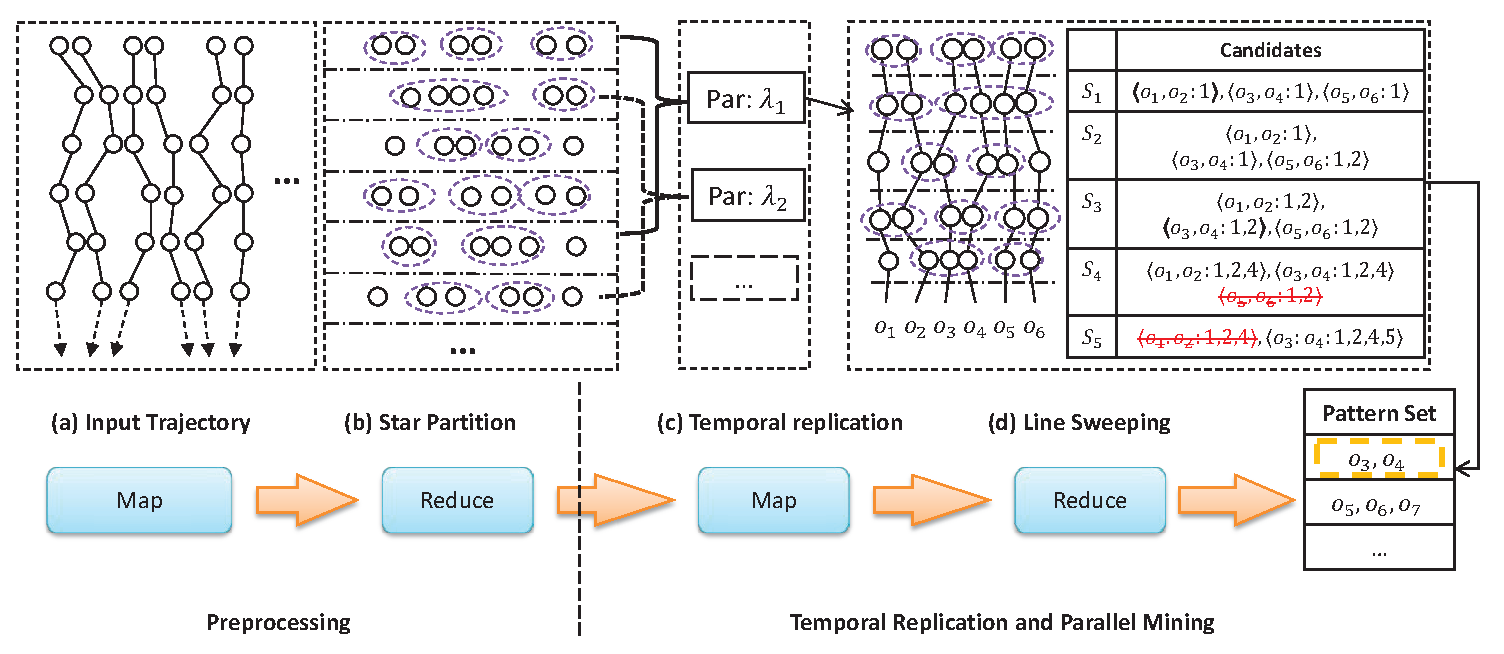
\includegraphics[width=\textwidth]{trm.eps}
\caption{Work flow of Temporal Replication and Mining. (a)(b) correspond to the first MR job which computes the clusters at each snapshot; 
(c)(d) correspond to the second MR job which uses TRM to mine GCMP in parallel.}
\label{fig:trm}
\end{figure*}

Since in the first MR job, each partition contains only one snapshot
for clustering, it is not necessary to replicate any snapshot. Thus, we
focus on describing the second MR job which is the \emph{Temporal
Replication and Mining} algorithm. We use $R$ to denote the replication factor.
The outline of TRM is 
shown in Algorithm~\ref{algo:trm_overview}.

\begin{algorithm}
\caption{Temporal Replication and Mining}
\label{algo:trm_overview}
\begin{algorithmic}[1]
\Require list of $\langle t, S_t \rangle$ pairs
\State $R \gets (\lceil \frac{K}{L} \rceil -1)*G+2K$
\State {---Map Phase---}
\label{code:trm-map-start}
\ForAll{$\langle t, S_t \rangle$}
	\ForAll{$i \in 1...R$}
		\State emit a $\langle t-i, S_t \rangle$ pair
	\EndFor  
\EndFor
\label{code:trm-map-end}
\State {---Partition and Shuffle Phase---}
\label{code:trm-par-start}
\ForAll{$\langle t, S \rangle$ pair} 
\State group-by $t$, emit a $\langle t, Par_t\rangle$
\State where $Par_t = \{S_t, S_{t+1}, .. S_{t+R}\} $
\EndFor
\label{code:trm-par-end}
\State {---Reduce Phase---}
\label{code:trm-red-start}
\ForAll{$\langle t,Par_t \rangle$}
\State lineSweepMining($Par_t$)
\label{code:trm-red-end}
\EndFor
\end{algorithmic}
\end{algorithm}

As shown in Algorithm~\ref{algo:trm_overview}, the TRM algorithm contains
three steps. First, in the map phase, each snapshot is keyed 
with its timestamp (lines~\ref{code:trm-map-start}-\ref{code:trm-map-end}). 
Second, in the partition phase, every snapshot is grouped with its next 
$R$ snapshots to form a partition (lines~\ref{code:trm-par-start}-\ref{code:trm-par-end}). 
We will shortly discuss how the $R$ value is derived. 
Third, in the reduce phase, a line sweeping method is invoked 
to mine GCMP within each partition (lines~\ref{code:trm-red-start}-\ref{code:trm-red-end}). 
It is easy to see that this method replicates a snapshots at most $R$ times.
%\subsubsection{Temporal Replication Partition}
The replication factor $R$ is critical for the performance of TRM.
If the $R$ is large, the shuffle cost as well as the reduce cost would be high. 
On the contrary, if $R$ is small, valid patterns may
be missed out. In the Algorithm~\ref{algo:trm_overview}, the 
$R$ is chosen as $(\lceil \frac{K}{L} \rceil -1)*G+2K$. We will show
later the correctness of this value.

%In the Algorithm~\ref{algo:trm_overview}, 
%the partition size is chosen as $(\lceil \frac{K}{L} \rceil -1)*G+2K$. As stated in the following
%theorem, such a partition method is sound and complete.
%\begin{theorem}[Soundness and Completeness of Replication]
%\label{thm:replication_partition}
%Let $\mathbb{P}$ be as follows: for each snapshot $S_t$, create a partition $Par_t = \{S_t, ...,S_{t+(\lceil \frac{K}{L} \rceil - 1) *G+2K}\}$. Then $\mathbb{P}$ is sound and complete.
%\end{theorem}
%\begin{proof}
%The soundness of partition can be observed from the fact that each partition represents partial trajectories with consecutive snapshots, therefore patterns in a partition can be directly mapped back to original trajectories.
%Given a valid pattern $P$, let $T' \subseteq P.T$ be the subsequence of $P.T$ which conforms to $K,L,G$ with the smallest size. Note that there could be many qualified $T'$s.  
%Let the $i^{th}$ local-consecutive part of $T'$ be $l_i$ and let the $i^{th}$ gap of $T'$ be $g_i$. Then, the size of $T'$ can be written as $\Sigma_i (l_i + g_i)$. 
%Since $T'$ conforms to $K,L,G$, then $2K \geq \Sigma_i (l_i) \geq K$, $l_i \geq L$, $g_i \leq G$. Therefore, $\Sigma_i(l_i+g_i) \leq (\lceil \frac{K}{L} \rceil -1) *G+2K$. Thus ensuring each $Par_t$ to be of that size would capture at least one of the $T'$s, therefore the pattern $P$ would be valid in $Par_t$. This proves the completeness of the partitioning method.
%\end{proof}

\subsection{Line Sweep Mining}
Each task in the reduce phase processes a partition $Par_i$, which contains
$R$ snapshots starting from snapshot $S_i$. We observe that within each $Par_i$, 
only the patterns whose object sets are contained in the first snapshot 
are necessary to be reported. Therefore, we design a simple 
\emph{line-sweep mining}(LSM) method for discovering
GCMPs. The algorithm works as in Algorithm~\ref{algo:line-sweep}.

\begin{algorithm}
\caption{Line Sweep Mining}
\label{algo:line-sweep}
\begin{algorithmic}[1]
\Require $Par_t = \{S_t, S_{t+1}, ...\}$
\State{$C \gets \{\}$} \Comment{Candidate set} \label{code:ls-can-set}
\For{$c \in S_t$} 
\label{code:ls-init-start}
\State $C$.add($\langle c, t \rangle $)
\EndFor
\label{code:ls-init-end}
\ForAll{$i \in [1,R]$}
\State $N \gets S_{t+i} \oplus C$ \label{code:ls-join}
	\ForAll {$n \in N$}
		\If{$|n.O| \geq M$}
			$C$.add($n$).
			\label{code:ls-add}
		\EndIf
	\EndFor
\State{remove unqualified candidate from $C$}
	\label{code:ls-remove}
\EndFor
\State{output qualified candidate in $C$}
\end{algorithmic}
\end{algorithm}

The algorithm scans snapshots in a partition in sequence. During the scan, it
maintains a candidate set $C$ which contains potential patterns (line~\ref{code:ls-can-set}).
The algorithm starts by inserting clusters at $S_i$ to $C$ (lines~\ref{code:ls-init-start}-\ref{code:ls-init-end}).
Subsequently, in each iteration, clusters in $C$ are joined with clusters at $S_i$ to generate
a new set of patterns $N$(lines~\ref{code:ls-join}). The valid new patterns 
form a new candidate set $C$ and any invalid patterns are discarded(lines~\ref{code:ls-add} and~\ref{code:ls-remove}).

%\begin{figure}[h]
%\centering
%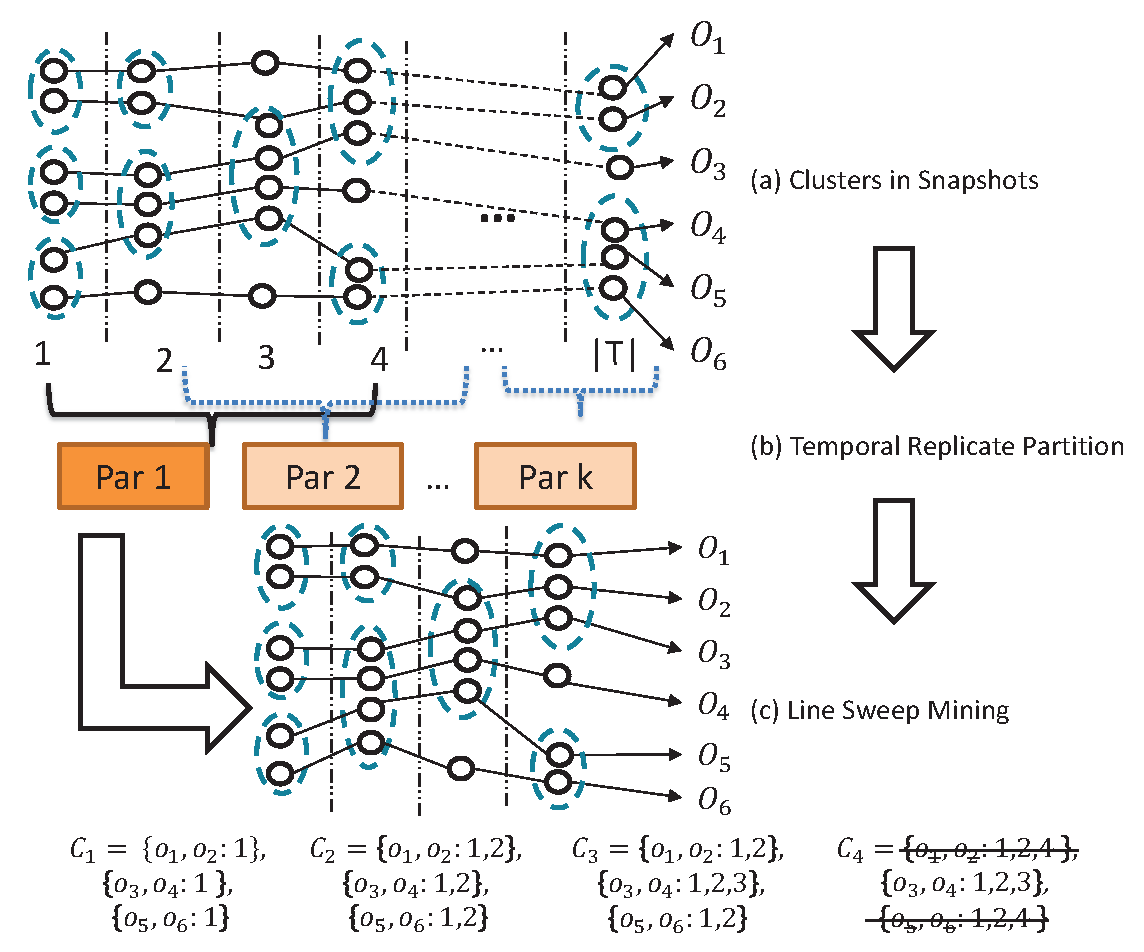
\includegraphics[width=0.5\textwidth]{trm_process.eps}
%\caption{Work flow of trajectory replication and mining}
%\label{fig:trm_process}
%\end{figure}

\subsection{Correctness of TRM}
We prove the correctness of TRM from two aspects. First,
the choice of $R = (\lceil \frac{K}{L} \rceil -1)*G+2K$ would 
not miss out any valid patterns. Second, no false patterns
are reported in any partitions. We formalize these two 
properties as \emph{completeness} and \emph{soundness} as follows:

\begin{definition}[Completeness and Soundness]
Let a partition method $\mathbb{P}$ partitions a trajectory database $Tr$ 
into segments, $Par_1,...,Par_m$. $\mathbb{P}$ is complete 
if for every valid pattern $P$ in $Tr$, $\exists Par_i$ s.t. $P$ is valid in $Par_i$. 
$\mathbb{P}$ is sound if for all patterns that are valid in any $Par_i$, they are also valid in $TR$.
\end{definition}

Apparently, in TRM, replicating the entire trajectories (i.e., $R=\mathbb{|T|}$)
meets the \emph{soundness} and \emph{completeness} requirements. However, it burdens the network shuffle and limits the parallelism. We carefully chose $R = (\lceil \frac{K}{L} \rceil -1)*G+2K$ and use
the following theorem to state the correctness:

\begin{theorem}[Correctness of Replication]
\label{thm:replication_partition}
Temporal replication partition is sound and complete.
\end{theorem}
\begin{proof}
The soundness of partition can be observed from the fact 
that each partition represents a consecutive segments of trajectories. 
Therefore patterns in a partition can be directly mapped 
back to original trajectories. For completeness, with a
valid pattern $P$, let $T'$ be the subsequence of $P.T$ which conforms to $K,L,G$ 
with the smallest length. Note that there could be many qualified $T'$s. 
Let the $i^{th}$ local-consecutive segment of $T'$ be $l_i$ and 
let the $i^{th}$ gap of $T'$ be $g_i$. Then, the size of $T'$ can 
be written as $\Sigma_i (l_i + g_i)$.  Since $T'$ conforms to $K,L,G$, 
then $2K \geq \Sigma_i (l_i) \geq K$, $l_i \geq L$, $g_i \leq G$. 
It follows: $\Sigma_i(l_i+g_i) \leq (\lceil \frac{K}{L} \rceil -1) *G+2K$. 
If every partition is of at least such a size, then $T'$ must be
captured by at least one of the partition. Thus, the pattern $P$ would 
be valid in that partition. This proves the completeness.
\end{proof}

\begin{example}
We illustrate the entire TRM method using Figure~\ref{fig:trm} (c)(d) with $M=2, K=2, L = 2, G=2$. 
In Figure~\ref{fig:trm} (c), snapshots are combined into partitions with sizes equal to 
$(\lceil \frac{K}{L} \rceil-1) *G+2K = 4$. Then a line sweep method is performed in (d) 
for partition $1$. Each $C_i$ refers to the candidate set during sweeping snapshot $i$. 
Initially, $C_1$ contains patterns whose object set is in snapshot $1$.
As line sweeps, at snapshot $4$, since the timestamps of $\{o_1,o_2\}$ and $\{o_5,o_6\}$ 
are both $\{1,2,4\}$ which violate the $G$ constraint, 
thus the two candidates are removed from $C_4$. After all snapshots are swept, 
$\{o_3,o_4\}$ is the qualified pattern and is outputted.
\end{example}

The TRM approach though achieves good parallelism, 
it requires to replicate the data multiple times. 
Specifically, each snapshots are replicate $(\lceil \frac{K}{L} \rceil -1) *G+2K$ times. 
In the cases of \emph{swarm}, \emph{group} and \emph{platoon}, $G$ is as large as $|T|$. 
Handling those cases is equivalent to replicate the entire snapshots to each partition, 
which surrenders the benefit of parallelism.



%IMPORTANT!!!
%In contrast, it is challenging to design the second job. 
%This is because valid patterns may spray across multiple snapshots 
%or contain different object sets, where inappropriate partitioning
%of snapshots may fail to discover certain valid patterns.
%Formally, a valid partition strategy 
%needs to meet the following requirements: (a) the resulted partitions need
%to preserve enough information so that real patterns can be discovered in the reduce phase. 
%(b) the resulted partitions need to ensure that
%the patterns discovered in the reduce phase are valid patterns so that
%no further verification is required. We formalize these two 
%properties as \emph{completeness} and \emph{soundness} as follows:
%
%\begin{definition}[Completeness and Soundness]
%Let a partition method $\mathbb{P}$ partitions original trajectories $Tr$ into multiple parts, $Par_1,...,Par_m$. $\mathbb{P}$ is complete if for every pattern $P$ that is valid in $Tr$, $\exists Par_i$ s.t. $P$ is valid in $Par_i$. $\mathbb{P}$ is sound if for all patterns that are valid in any $Par_i$, they are also valid in $TR$.
%\end{definition}
%The completeness ensures that no true patterns are missed out. 
%The soundness ensures that no false patterns are reported. 
%If a partition method is both sound and complete, then it can be used
%in the second MR job to facilitate GCMP mining.
%
%Apparently, replicating the entire trajectories to each 
%partition meets the \emph{soundness} and \emph{completeness} requirements. 
%However, it burdens the network shuffle and limits the parallelism. 
%Our objective is thus to design a complete and sound partition method that minimize the network shuffles.
%In the following sections, we describe a naive \emph{temporal-based} partition-and-mining method called \emph{Temporal Replication and Mining}(TRM) towards a parallel solution of GCMP mining. Then,
%we present a novel \emph{object-based} partition-and-mining method
%called \emph{Star Partition and Mining} (SPM) which resolves
%the deficiencies of TRM method.

\section{Temporal Replication and Mining}
\label{sec:trm_solution}
The idea of \emph{Temporal Replication and Mining} (TRM)
is to group temporally contiguous snapshots together, s.t. patterns can be
mined from each group of snapshots. In order to achieve the \emph{completeness}
and \emph{soundness} during partitioning, we allow replication of
snapshots among groups. The TRM is outlined in Algorithm~\ref{algo:trm_overview}.

\begin{algorithm}
\caption{Temporal Replication and Mining}
\label{algo:trm_overview}
\begin{algorithmic}[1]
\Require list of $\langle t, S_t \rangle$ pairs
\State {---Map Phase---}
\label{code:trm-map-start}
\ForAll{$\langle t, S_t \rangle$}
	\ForAll{$i \in 1...(K-1)*G+K$}
		\State emit a $\langle t-i, S_t \rangle$ pair
	\EndFor 
\EndFor
\label{code:trm-map-end}
\State {---Partition and Shuffle Phase---}
\label{code:trm-par-start}
\ForAll{$\langle t, S \rangle$ pair} 
\State group-by $t$, emit a $\langle t, Par_t\rangle$,
\State  where $Par_t = \{S_t, S_{t+1}, .. S_{t+(\lceil \frac{K}{L} \rceil -1)*G+2K}\} $
\EndFor
\label{code:trm-par-end}
\State {---Reduce Phase---}
\label{code:trm-red-start}
\ForAll{$\langle t,Par_t \rangle$}
\State lineSweepMining($Par_t$)
\label{code:trm-red-end}
\EndFor
\end{algorithmic}
\end{algorithm}

As shown in Algorithm~\ref{algo:trm_overview}, the TRM algorithm contains
three steps. First, in the map phase, each snapshot is keyed 
with its timestamp (lines~\ref{code:trm-map-start}-\ref{code:trm-map-end}). 
Second, in the partition phase, every snapshot is grouped with its next 
$(\lceil \frac{K}{L} \rceil -1)*G+2K$ snapshots to form a partition (lines~\ref{code:trm-par-start}-\ref{code:trm-par-end}). We will shortly discuss how the group size is derived. 
Third, in the reduce phase, a lineSweepMining method is invoked 
to mine GCMP within each partition (lines~\ref{code:trm-red-start}-\ref{code:trm-red-end}). 
It is easy to see that this method replicates a snapshots 
at most $(\lceil \frac{K}{L} \rceil -1)*G+2K$ times.

\subsubsection{Temporal Replication Partition}
The size of replication is critical for the performance of TRM algorithm.
If the size of replication is too large, the shuffle cost as well as the reduce cost would be high. 
On the contrary, if the size of replication is too small, the \emph{completeness} and \emph{soundness}
properties cannot be satisfied. In the Algorithm~\ref{algo:trm_overview}, 
the partition size is chosen as $(\lceil \frac{K}{L} \rceil -1)*G+2K$. As stated in the following
theorem, such a partition method is sound and complete.
\begin{theorem}[Soundness and Completeness of Replication]
\label{thm:replication_partition}
Let $\mathbb{P}$ be as follows: for each snapshot $S_t$, create a partition $Par_t = \{S_t, ...,S_{t+(\lceil \frac{K}{L} \rceil - 1) *G+2K}\}$. Then $\mathbb{P}$ is sound and complete.
\end{theorem}
\begin{proof}
The soundness of partition can be observed from the fact that each partition represents partial trajectories with consecutive snapshots, therefore patterns in a partition can be directly mapped back to original trajectories.
Given a valid pattern $P$, let $T' \subseteq P.T$ be the subsequence of $P.T$ which conforms to $K,L,G$ with the smallest size. Note that there could be many qualified $T'$s.  
Let the $i^{th}$ local-consecutive part of $T'$ be $l_i$ and let the $i^{th}$ gap of $T'$ be $g_i$. Then, the size of $T'$ can be written as $\Sigma_i (l_i + g_i)$. 
Since $T'$ conforms to $K,L,G$, then $2K \geq \Sigma_i (l_i) \geq K$, $l_i \geq L$, $g_i \leq G$. Therefore, $\Sigma_i(l_i+g_i) \leq (\lceil \frac{K}{L} \rceil -1) *G+2K$. Thus ensuring each $Par_t$ to be of that size would capture at least one of the $T'$s, therefore the pattern $P$ would be valid in $Par_t$. This proves the completeness of the partitioning method.
\end{proof}

\subsubsection{Line Sweep Mining}
After partition, each task in the reduce phase processes a partition $Par_i$, which contains
$(\lceil \frac{K}{L} \rceil -1) *G+2K$ snapshots starting from snapshot $S_i$. With such a 
partition method, we observe that within $Par_i$, only the 
patterns whose object sets are contained in the first snapshot are necessary to be reported.
Therefore, we design a simple \emph{line-sweep mining}(LSM) method for discover
GCMPs. The algorithm works as in Algorithm~\ref{algo:line-sweep}.

\begin{algorithm}
\caption{Line Sweep Mining}
\label{algo:line-sweep}
\begin{algorithmic}[1]
\Require $Par_t = \{S_t, S_{t+1}, ...\}$
\State{$C \gets \{\}$} \Comment{Candidate set} \label{code:ls-can-set}
\For{$c \in S_t$} 
\label{code:ls-init-start}
\State $C$.add($\langle c, t \rangle $)
\EndFor
\label{code:ls-init-end}
\For{$i=1; i < |Par_t|;i++$}
\State $N \gets S_i \oplus C$ \label{code:ls-join}
	\ForAll {$n \in N$}
		\If{$|n.O| \geq M$}
			$C$.add($n$).
			\label{code:ls-add}
		\EndIf
	\EndFor
\State{remove unqualified candidate from $C$}
	\label{code:ls-remove}
\EndFor
\State{output qualified candidate in $C$}
\end{algorithmic}
\end{algorithm}

The algorithm scans the snapshots in a partition in sequential order. During the scan, it
maintains a candidate set $C$ which could potentially be a valid pattern (line~\ref{code:ls-can-set}).
The algorithm starts by inserting clusters at $S_1$ to $C$ (lines~\ref{code:ls-init-start}-\ref{code:ls-init-end}).
Subsequently, in each iteration, clusters in $C$ are joined with clusters at $S_i$ to generate
a new set of patterns $N$(lines~\ref{code:ls-join}). Any valid new patterns are inserted back to $C$
and any invalid patterns are discarded(lines~\ref{code:ls-add} and~\ref{code:ls-remove}).

\begin{figure}[h]
\centering
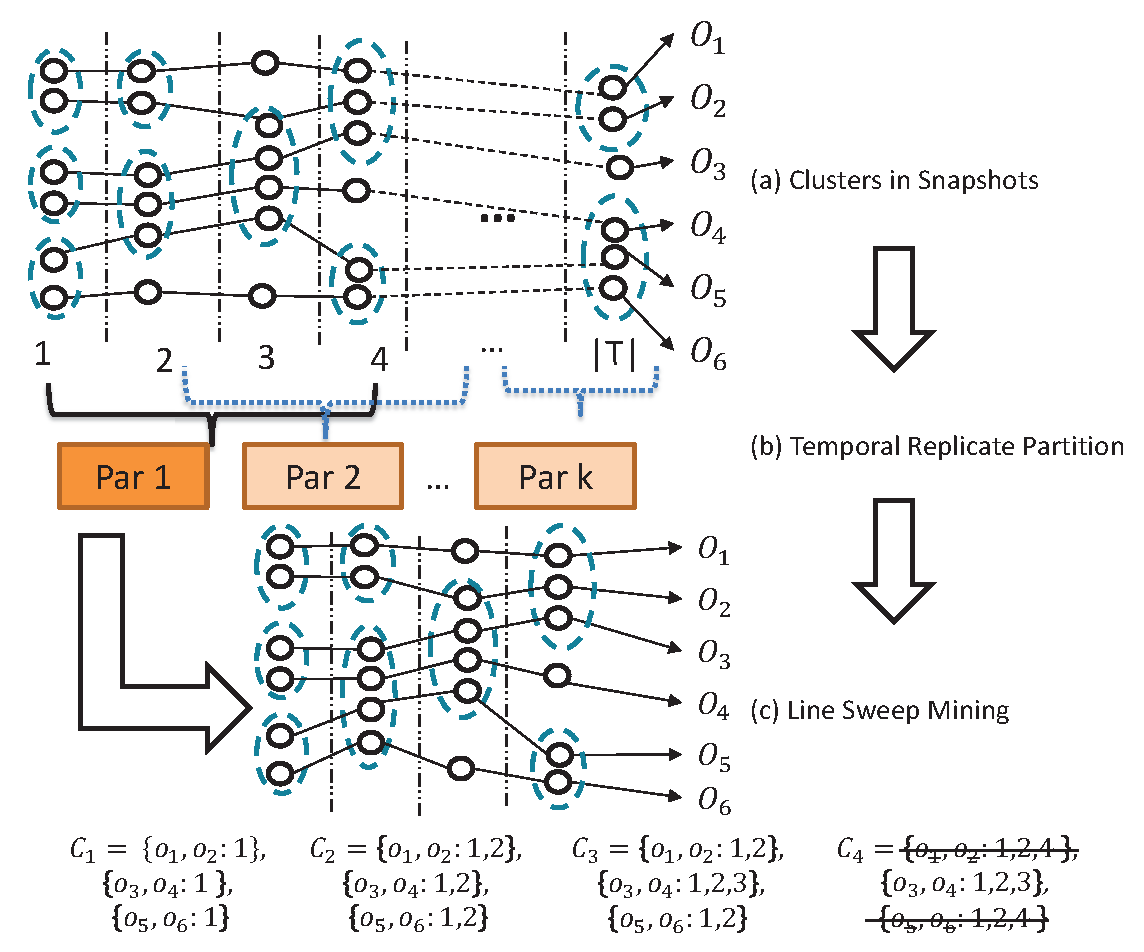
\includegraphics[width=0.5\textwidth]{trm_process.eps}
\caption{Work flow of trajectory replication and mining}
\label{fig:trm_process}
\end{figure}

\begin{example}
We illustrate the process of TRM in Figure~\ref{fig:trm_process} using $M=2, K=2, L = 2, G=2$. In (a), snapshots are clustered and these snapshots are the input to the TRM. Then, we compute the size 
for each partition, which equals to $(\lceil \frac{K}{L} \rceil-1) *G+2K = 4$. Therefore, in (b), every four snapshots
are grouped into a partition. Then a line sweep method is performed in (c) for partition 1. Each
$C_i$ refers to the candidate set  when the algorithm sweeps each snapshot. Initially, $C_1$ contains
patterns whose object set is in $S_1$. When scanning the other snapshots, patterns in $C_1$ grow
their timestamps. At $S_3$, since the timestamps of $\{o_5,o_6\}$ is $\{1\}$ which is neither
a qualified pattern nor matches $G$ constraint, thus this candidate is removed from $C_3$. When line
sweep finishes, only $\{o_3,o_4\}$ is the qualified pattern and is outputted.
\end{example}


The TRM approach though achieves good parallelism, 
it requires to replicate the data multiple times. 
Specifically, each snapshots are copied $(\lceil \frac{K}{L} \rceil -1) *G+2K$ times. 
In the cases of \emph{swarm}, \emph{group} and \emph{platoon}, $G$ is as large as $|T|$. 
Handling those cases is equivalent to replicate the entire snapshots to each partition, 
which surrenders the benefit of parallelism.


\section{Star Partition and Mining}
\label{sec:spm_solution}
In order to achieve a good parallelism 
under any pattern parameters, we propose 
the \emph{Star Partition and Mining} (SPM) method. 
In SPM, we first design a novel object-based partition 
method named \emph{star partition}. Then, we adapt
an \emph{Apriori} method to mine GCMP patterns
out of each partition. 


 The overview of the SPM method 
is presented in Algorithm~\ref{algo:spm_overview}.
As shown, the SPM method takes three phases. 
In the map phase, objects from the same cluster forms object-object pairs. 
The object-object pairs are then paired up with the timestamp of 
the snapshot to form a triplet(lines~\ref{code:spm-map-start}-\ref{code:spm-map-end}). 
In the partition phase, triplets with the same leading object form a \emph{star} which will be explained shortly 
(lines~\ref{code:spm-shuffle-start}-\ref{code:spm-shuffle-end}).
Lastly in the reduce phase, patterns are mined from each star structure (lines~\ref{code:spm-reduce-start}-\ref{code:spm-reduce-end}).

\begin{algorithm}
\caption{Star Partition and Mining}
\label{algo:spm_overview}
\begin{algorithmic}[1]
\Require list of $\langle t, S_t \rangle$ pairs
\State {---Map phase---}
\label{code:spm-map-start}
\ForAll{$C \in S_t$}
	\ForAll {$(o_1 ,o_2) \in C \times C$}
		\If{$o_1 < o_2$}  \label{code:spm-edge-direct}
			\State emit a $\langle o_1, o_2, \{t\}\rangle$ triplet
		\EndIf
	\EndFor
\EndFor
\label{code:spm-map-end}

\State {---Partition and Shuffle phase---}
\label{code:spm-shuffle-start}
\ForAll{$\langle o_1, o_2, \{t\}\rangle$ triplets} 
	\State group-by $o_1$, emit $\langle o_1, Sr_{o_1} \rangle$ 
	%\State group-by $o_2$, emit $\langle o_2, Sr_{o_2} \rangle$
\EndFor
\label{code:spm-shuffle-end}

\State {---Reduce phase---}
\label{code:spm-reduce-start}
\ForAll{$\langle o, Sr_{o} \rangle$}
\State Apriori($Sr_o$)
\EndFor
\label{code:spm-reduce-end}

\end{algorithmic}
\end{algorithm}

\subsection{Star Partition}
The intuition of the star partition is that, if two objects are part 
of the same pattern, they must belong to the same cluster at 
some snapshots. Therefore, we may link objects that belong to the same cluster to form a \emph{connection graph}. Objects that are
not connected surely fail to form a pattern. We may then
partition the connection graph based on vertex connectivity
s.t. mining GCMPs can be done in parallel. We define the \emph{connection graph} and \emph{star}
as follows:
\begin{definition}[Connection Graph and Star]
A connection graph is an undirected graph $G=(V:E)$, where 
each $v \in V$ represents an object. An edge $e(s,t)= ET \in E$ 
contains all the timestamps at which $s,t$ are in the same cluster,
i.e., $\forall t \in ET, C_t(s) = C_t(t)$. 
A star of a vertex $s$, denoted as $Sr_s$, is the set of incidental edges on $s$ whose
another ending vertex is greater than $s$. I.e, $\forall e(s,t) \in Sr_s$, $s < t$. We name $s$
as the \emph{central vertex} of $Sr_s$.
\end{definition}

It is notable that we require vertices in a star to be greater than its central vertex. This 
effectively avoids replicating edges. \emph{Connection graph} and \emph{star} examples are 
shown in Figure~\ref{fig:star_partition} (a) and (b). In (a), a connection graph is formed
based on the example in Figure~\ref{fig:related_work}.
In (b), 5 stars are presented. It is easy to see that, by requiring the center vertex to be
the smallest vertex in a star, there are no edges been replicated. In implementation,
as stated in Algorithm~\ref{algo:spm_overview} line~\ref{code:spm-edge-direct}, the
comparison between vertices/objects are based on the vertex/object ID.

\begin{figure*}[t]
\centering
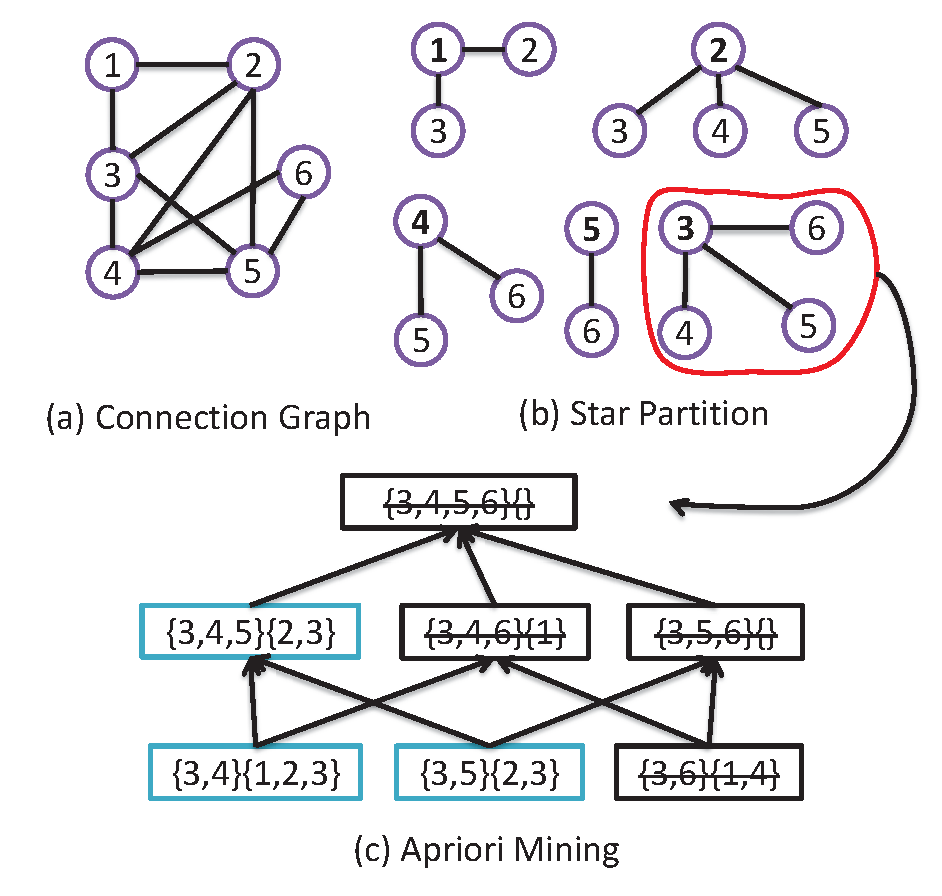
\includegraphics[width=0.9\textwidth]{spm.eps}
\caption{Star partition and mining. (a) Conceptual connection graph from Figure 1.(b) Five star partitions are generated
(c) Apriori Mining with various pruning techniques.}
\label{fig:star_partition}
\end{figure*}

%After computing the star, each partition is applied with a reduce task. 
%Indeed, a star $Sr_s$ can be viewed as a subset of original trajectories. 
%This is done by treating each vertex in $Sr_s$ as an object. 
%The time sequence of $s$ is the union of all edges in $Sr_s$. 
%And the time sequence of $v \neq s$ is the edge $(s,v)$. Therefore, we
%are able to mine stars from the similar trajectory concepts.
Although star partition is performed based on the object connections, each star
can be effectively viewed as a subset of trajectories. To see this, each vertex
in a star can be viewed as an object. The timestamps of center vertex $s$ is the
union of all the edges in $Sr_s$. The timestamps of vertex $v \neq s$ is the 
edge $e(s,v)$. Therefore, we are able to define and mine GCMP on the stars. 
Before describing the mining strategy, we first state in the following theorem that 
the star-partition is complete and sound:
\begin{theorem}[Soundness and Completeness of Star Partition]
Star partition is sound and complete.
\end{theorem}

\begin{proof}
For the soundness,
if $P$ is a valid pattern in $Sr_s$, then at every time $t$, $\forall o_1, o_2 \in P.O$, $C_t(o_1) = C_t(o_2)$.
By definition, $P$ is valid in the original trajectories.
For the completeness,
if $P$ is a valid pattern in original trajectories, let $s$ be the object with smallest ID in $P.O$. 
Then by the definition of pattern, $\forall t \in P.T$, $\forall o \in P.O$, $C_t(s) = C_t(o)$.
It follows that all object $o \in P.O$ are in $Sr_s$. Furthermore, every timestamp in $P.T$ is included
in $Sr_s$. Therefore, $P$ is a valid pattern in $Sr_s$.
\end{proof}

Based on the above theorem, we can mine GCMP from each partition independently.
It is notable that, in star partition, original data is replicated for $O(|\mathbb{O}|)$ times
as each object may be sent to $O(|\mathbb{O}|)$ partitions. Since this complexity is free
from pattern parameters, the star partition is more scalable than the temporal replication.
In later sections, we will describe several engineering level optimization to further reduce the amount of replicated data.

\subsection{Apriori Mining}
In the mining phase, we need to find the patterns within each star. 
To systematically discover the patterns, we design the \emph{Apriori Mining} method which
is similar to the technique in frequent item mining literature. During the algorithm, we call a candidate pattern $R$-pattern if the size of its object set is $R$. 
Our algorithm runs in iterations. During each iteration $R$, we try to generate all $(R+1)$-patterns. In iteration $1$, the $2$-pattern is the edges in $Sr_s$. In particular,
for each $e(s,v)=ET$, pattern $p=(\{s,v\}, ET)$ is formed. During each iteration, 
we generate $(R+1)$-patterns by joining $R$-patterns with $2$-patterns. Specifically,
the join between $p_1=(O_1:T_1)$ and $p_2=(O_2:T_2)$ would generate a new pattern $p_3=(O_1 \cup O_2:T_1 \cap T_2)$. Notice that in $Sr_s$, each $R$-pattern consists of the object $s$, thus the join will grow a $R$-pattern at most to a $(R+1)$-pattern.
Our mining algorithm stops where no further patterns are generated. The algorithm is illustrated as in Algorithm~\ref{algo:apriori_mining}.

\begin{algorithm}
\caption{Apriori Mining}
\label{algo:apriori_mining}
\begin{algorithmic}[1]
\Require{$Sr_s$}
\State { Lv $\gets \{\}$,Ground $\gets \{\}$, Output $\gets \{\}$}
\ForAll{$e(s,t) = T \in Sr_s$}
\State Ground.add($\langle \{s,t\}, T \rangle$);
\State Lv $\gets$ Ground;
\EndFor
\While{true}
	\If{Lv is not empty} 
		\State{LvCand $\gets \{\}$ }
		\ForAll{$cand_v \in Lv$}
			\ForAll{$cand \in $Ground}
				\State $p \gets cand_v$ join $cand$
				\If{$p.T$ is a candidate sequence} 
					\State LvCand.add($p$)
				\EndIf
			\EndFor
		\EndFor
		\If{$Lv$ is a pattern}
			\State{Output.add($Lv$)}
			\State{break}			 
		\EndIf
		\State {Lv $\gets$ LvCand}
	\Else
		\State{break}
	\EndIf
\EndWhile
\State output.addAll($Lv$)
\State \Return output
\end{algorithmic}
\end{algorithm}

An illustration of Algorithm~\ref{algo:apriori_mining} is shown in Figure~\ref{fig:star_partition} (c).
As shown, the star $Sr_3=\{3,4,5,6\}$ initially generate three $2$-candidates. At every iteration, 
higher level candidates are generated by joining lower level candidates. When no more candidates 
can be generated, the algorithm stops by outputting the valid patterns.

It is notable that Algorithm~\ref{algo:apriori_mining} takes exponential complexity to mine GCMP. There
are two major factors dragging down the performance. First, the size of $Sr_s$ affects
the initial size of $2$-patterns. Second, the candidates generated in each level affects the join performance. In later
sections, we exploit the property of GCMP to reduce the two factors.

\section{Optimization}
\label{sec:optimization}
In this section, we describe several optimizations to the star-partition and mining algorithm.
In addition, we also address some practical issues when deploying the SPM algorithm
to real MapReduce based systems.

%We have analyzed that the bottlenecks of Algorithm~\ref{algo:apriori_mining} 
%lies in two factors. The size of each $Sr_s$ and the size of candidates in each level of Apriori.
%In this section, we provide several optimizations to boost the bottlenecks.
%\subsection{Edge Reduction by Direction}
%The first spot for reducing the size of $Sr_s$ is to remove the replicated edges. As shown in Algorithm~\ref{algo:spm_overview}, each edge in the conceptual graph is replicated twice in generating the star-structure. The purpose of replication is to ensure the completeness of star partition. However, this replication can be avoided if we choose an appropriate way of partitioning. 
%
%We design the edge partitioning method by edge direction. Instead of building a conceptual graph that is undirected, we create the directed conceptual graph as follows: First, we assign each object a unique number. Then
%for a cluster $C_t$ in snapshot $S_t$, for any pair $(u,v) \in C_t$, an edge $e(u,v) = \{t\}$ is created if $u < v$. It is easy to see that the directed conceptual graph is a DAG. We then create each $Sr_u$ by including all the outgoing edges of $u$. By so doing, each edge is assigned to only one star, thus avoids the replications. We use the following theorem to ensure the completeness of the edge direction method.
%
%\begin{theorem}[Sound and Completeness of Edge Direction]
%Star partition with edge direction is sound and complete.
%\end{theorem}
%\begin{proof}
%It is notable that each star is a subset of original trajectories, thus the soundness is trivially true. For completeness, if $P$ is valid pattern, then let $s$ be the object of the smallest number in $P.O$, i.e., $s=\min_{o \in P.O}(o)$. Since $s$ is smallest and the all other objects in $P.O$ is connected with $s$. Therefore, $P.O \equiv Sr_s$, which indicates that $P.O$ is also a pattern in $Sr_s$.
%\end{proof}
%An example of edge direction is shown in Figure~\ref{fig:star_partition}. As shown,
%by adapting the direction method, half the size of $S_r$'s is reduced. This clearly brings efficiency in both shuffling and apriori mining.

\subsection{Edge Simplification}
Each edge $e(s,v)$ in $Sr_s$ contains a time sequence $ET$ 
which represents the co-occurrence of $s$ and $v$. We notice that the edge 
between $s$ and $t$ is not always necessary. For example, if an edge has a
cardinality less than $K$, it is unnecessary to include this edge to 
$Sr_s$ since it cannot contribute to any patterns.
This motivates us to simplify the edges in $Sr_s$ 
to boost the overall performance.

Our goal of edge simplification is to, given a time sequence $T$, find a subsequence
of $T' \subseteq T$, such that $T'$ is potentially conforms to $K,L,G$. And we
wish $|T'|$ to be as small as possible.  
We star-off by observing that for every time sequence $T$, $T$ can be 
divided into a set of maximally $G$-connected subsequences. Note that
a maximally $G$-connected subsequence can potentially contribute to
a pattern if it conforms to $K,L$.
Therefore, we are able to reduce $T$
to its maximally $G$-connected subseuqnces which conform to $K,L$.

To formally describe the idea, we define the a \emph{candidate sequence} as follows:

%\begin{definition}[Candidate Sequence]
%Given the pattern parameters: $K,L,G$, a sequence $T$ is 
%a \emph{partly candidate} sequence if exists one of its maximal $G$-connected
%subsequence $T'$ such that $T'$ confirms to $L,K$.
%\end{definition}

%For example, let $L = 2, K = 4, G = 2$, sequence $T_1=(1,2,4,5,6,9,10,11)$ 
%is a \emph{partly candidate sequence} since $T_1[1:5] = (1,2,4,5,6)$ is a valid
%pattern wrt. $L,K,G$. In contrast, $T_2=(1,2,5,6,7)$ is not a valid partly candidate sequence.
%
%Observing that only partly candidate sequence can be potentially contribute to a 
%pattern. Therefore, given an edge $e(s,t)=T \in Sr_s$, if $T$ is not a partly
%candidate sequence, it can be pruned from $Sr_s$. To efficiently
%test whether a given sequence is partly candidate, we define the \emph{Fully Candidate Sequence}:

\begin{definition}[Candidate Sequence]
Given the pattern parameters: $L,K,G$, a sequence $T$ is a \emph{Candidate Sequence} 
if for any of its maximal $G$-connected sequence $T'$, $T'$ conforms to $L,K$.
\end{definition}

For example, let $L = 2, K = 4, G = 2$, sequence $T_1=(1,2,4,5,6,9,10,11,13)$ is 
not a fully candidate sequence since one of its maximal $G$-connected sequence $(9,10,11)$
is not a partly candidate sequence. In contrast, sequence $T_2=(1,2,4,5,6)$ is 
a fully candidate sequence.

To reduce a sequence $T$ to a candidate sequence, we need to strip out its 
maximal $G$-connected subsequences which does not form to $K,L$. Such a reduction
takes two rounds scan of $T$ as shown in Algorithm~\ref{algo:simp_prune}. In the 
first round, the consecutive portions of $T$ with size less than $L$ are removed.
In the second round, the maximal $G$-connected sequences of size less than $K$ are
removed. Clearly the simplification algorithm runs in $O(|T|)$ time.
\begin{algorithm}
\caption{Edge Simplification}
\label{algo:simp_prune}
\begin{algorithmic}[1]
\Require $T$
\State{---Remove the consecutive portion with size less than $L$---}
\State $c \gets 0$
\For {$i \in (0,...,|T|)$}
	\If{$T[i] - T[i-1] != 1$} 
		\If{$i - c < L$} 
			\State $T$ remove $[c:i)$
		\EndIf
		\State $c \gets i$
	\EndIf
\EndFor
\State{---Remove the pseduo-consecutive portion with size less than $K$---}
\State $s\gets 1$, $c\gets 0$
\For{$i \in (0: |T|)$}
	\If{$T[i] - T[i-1] > G$}
		\If{$s < K$}   
			\State $T$ remove $[c:i)$
		\EndIf
		\State {$c \gets i$, $s \gets 1$}
	\Else
		\State $s++$
	\EndIf
\EndFor
\end{algorithmic}
\end{algorithm}

\begin{example}
Take $T_1=\{1,2,4,5,6,9,10,11,13\}$ as an example of edge simplification. Let $L = 2, K = 4, G = 2$.
In the first round of scan. $T_1$ reduces to $\{1,2,4,5,6,9,10,11\}$. The consecutive subsequence $\{13\}$
is removed by $L=2$. $T_1$ has two maximal $G$-consecutive subsequences, which 
are $\{1,2,4,5,6\}$ and $\{9,10,11\}$. Since $K=4$, $\{9,10,11\}$ is removed
from $T_1$ in the second round of scan. Therefore, $T_1$ is simplified to $\{1,2,4,5,6\}$.
\end{example}

%
%Based on the fully candidate sequence, we can reduce an sequence $T$ to a 
%fully candidate sequence by striping out its non-partly candidate maximal pseudo-consecutive 
%sequences. The reduction works as in Algorithm~\ref{algo:simp_prune}. It takes two
%rounds of scan of an input $T$. In the first round of scan,
%the consecutive portion of $T$ with size less than $L$ is removed.
%In the second round of scan, the pseudo-consecutive portion of $T$ with size less than $K$
%is removed. 


By leveraging the edge simplification technique, 
the size of the edges in $Sr_s$ can be greatly reduced. If
an edge cannot be reduced to a candidate sequence, then it is directly removed from $Sr_s$.
If an edge can be reduced to a candidate sequence, replacing itself 
by the candidate sequence results in a more compact storage.

%We use the following theorem to state the completeness and correctness of the 
%edge reduction algorithm.
%\begin{theorem}[Soundness and Completeness Edge Simplification]
%Star partition with edge simplification is sound and complete.
%\end{theorem}
%
%\begin{proof}
%Soundness of the star partition is not affected by edge simplification since each star is a subset of original trajectory. For completeness, notice that given a time sequence $T$, and any of its maximal $G$-connected subsequence $T'$, if $T'$ does not conform to $L,K$, then $T'$ cannot contribute to any patterns. 
%\end{proof}


\subsection{Candidate Pruning}
\subsubsection{Temporal monotonicity}
During the apriori phase, we repeatedly join candidate patterns in different levels to generate a larger set
of a patterns. We observe that traditional monotonic property of Apriori algorithms \textbf{does not}
hold in GCMP mining. That is given two candidate $P_1, P_2$, if $P_1.O \subset P_2.O$ and $P_1$ is not 
a valid pattern, then $P_2$ may or may not be a valid pattern. However, we notice that
we may form another monotonic property based on the \emph{candidate sequence} such that
the Apriori algorithm could still benefit.

The intuition is that if a candidate $P_1.T$ cannot be reduce to a \emph{candidate sequence}, then $P_1$ cannot 
be valid pattern. Furthermore, any candidate $P_2$, with $P_1.O \subset P_2.O$ cannot be a valid pattern.
This \emph{temporal monotonic property} 
is explicitly described as in the follow theorem:

\begin{theorem}[Temporal Monotonic Property of GCMP]
Given the temporal parameters $L,G,K$, for a candidate $c$ in Algorithm~\ref{algo:apriori_mining},
if $c.T$ cannot be reduced to a candidate sequence, then for any candidate $c'$ with $c.O \subset c'.O$, $c'$ can be pruned.
\end{theorem}
\begin{proof}
Let $c_1$, $c_2$ be two candidates with $c_1.O \subset c_2.O$. It is easy to see that $c_1.T \supseteq c_2.T$.
If $c_1.T$ cannot be reduced to a candidate sequence, then any subset of $c_1.T$ cannot
be reduced. It follows that $c_2.T$ cannot be reduced neither. Thus,
if $c_1.T$ cannot be reduced to a candidate sequence, $c_2$ can be pruned. 
\end{proof}

\subsubsection{Forward closure checking}

\begin{example}
We use Figure~\ref{fig:star_partition} (c) to demonstrate the candidate pruning. As shown, at the initial stage, $\{3,6:1,4\}$ is pruned, since $\{1,4\}$ is not a candidate sequence. By temporal monotonicity, candidates containing objects $\{3,6\}$ can all be pruned. Therefore, we are able to directly prune $\{3,4,6\}$, $\{3,5,6\}$ and $\{3,4,5,6\}$.
\end{example}
%
%With the help of the \emph{Monotonic Property}, the number of new candidates in each level is greatly reduced. We verify this in the experiment session as well.
\subsection{Load Balancing}

\subsection{Duplication Detection}

\subsection{Handling Overlapping Clusters}
\section{Experimental Study}
\label{sec:experiment}
\section{Conclusion and Future Work}
\label{sec:conclusion}

% The following two commands are all you need in the
% initial runs of your .tex file to
% produce the bibliography for the citations in your paper.
\bibliographystyle{IEEEtr}
\small
\bibliography{citations}
\end{document}
